%% 
%DIF LATEXDIFF DIFFERENCE FILE
%DIF DEL RES_droughts_Morin_ReEn.tex      Mon Jan 20 17:56:31 2025
%DIF ADD RES_droughts_Morin_ReEn_R3.tex   Mon Apr  7 18:08:01 2025
%% Copyright 2007-2025 Elsevier Ltd
%% 
%% This file is part of the 'Elsarticle Bundle'.
%% ---------------------------------------------
%% 
%% It may be distributed under the conditions of the LaTeX Project Public
%% License, either version 1.3 of this license or (at your option) any
%% later version.  The latest version of this license is in
%%    http://www.latex-project.org/lppl.txt
%% and version 1.3 or later is part of all distributions of LaTeX
%% version 1999/12/01 or later.
%% 
%% The list of all files belonging to the 'Elsarticle Bundle' is
%% given in the file `manifest.txt'.
%% 
%% Template article for Elsevier's document class `elsarticle'
%% with harvard style bibliographic references

\documentclass[preprint, 12pt]{elsarticle}

%% Use the options 1p,twocolumn; 3p; 3p,twocolumn; 5p; or 5p,twocolumn
%% for a journal layout:
%% \documentclass[final,1p,times,authoryear]{elsarticle}
%% \documentclass[final,1p,times,twocolumn,authoryear]{elsarticle}
%% \documentclass[final,3p,times,authoryear]{elsarticle}
%% \documentclass[final,3p,times,twocolumn,authoryear]{elsarticle}
%% \documentclass[final,5p,times,authoryear]{elsarticle}
%% \documentclass[final,5p,times,twocolumn,authoryear]{elsarticle}

%% For including figures, graphicx.sty has been loaded in
%% elsarticle.cls. If you prefer to use the old commands
%% please give \usepackage{epsfig}

%% The amssymb package provides various useful mathematical symbols
\usepackage{amssymb}
%% The amsmath package provides various useful equation environments.
\usepackage{amsmath}
%% The amsthm package provides extended theorem environments
%% \usepackage{amsthm}

%% The lineno packages adds line numbers.
\usepackage{lineno}

%% Use this package to add line brakes in URL
\usepackage{xurl}

\graphicspath{ {../Scripts/} }

\journal{Renewable Energy}
%DIF PREAMBLE EXTENSION ADDED BY LATEXDIFF
%DIF UNDERLINE PREAMBLE %DIF PREAMBLE
\RequirePackage[normalem]{ulem} %DIF PREAMBLE
\RequirePackage{color}\definecolor{RED}{rgb}{1,0,0}\definecolor{BLUE}{rgb}{0,0,1} %DIF PREAMBLE
\providecommand{\DIFadd}[1]{{\protect\color{blue}\uwave{#1}}} %DIF PREAMBLE
\providecommand{\DIFdel}[1]{{\protect\color{red}\sout{#1}}}                      %DIF PREAMBLE
%DIF SAFE PREAMBLE %DIF PREAMBLE
\providecommand{\DIFaddbegin}{} %DIF PREAMBLE
\providecommand{\DIFaddend}{} %DIF PREAMBLE
\providecommand{\DIFdelbegin}{} %DIF PREAMBLE
\providecommand{\DIFdelend}{} %DIF PREAMBLE
\providecommand{\DIFmodbegin}{} %DIF PREAMBLE
\providecommand{\DIFmodend}{} %DIF PREAMBLE
%DIF FLOATSAFE PREAMBLE %DIF PREAMBLE
\providecommand{\DIFaddFL}[1]{\DIFadd{#1}} %DIF PREAMBLE
\providecommand{\DIFdelFL}[1]{\DIFdel{#1}} %DIF PREAMBLE
\providecommand{\DIFaddbeginFL}{} %DIF PREAMBLE
\providecommand{\DIFaddendFL}{} %DIF PREAMBLE
\providecommand{\DIFdelbeginFL}{} %DIF PREAMBLE
\providecommand{\DIFdelendFL}{} %DIF PREAMBLE
%DIF LISTINGS PREAMBLE %DIF PREAMBLE
\RequirePackage{listings} %DIF PREAMBLE
\RequirePackage{color} %DIF PREAMBLE
\lstdefinelanguage{DIFcode}{ %DIF PREAMBLE
%DIF DIFCODE_UNDERLINE %DIF PREAMBLE
  moredelim=[il][\color{red}\sout]{\%DIF\ <\ }, %DIF PREAMBLE
  moredelim=[il][\color{blue}\uwave]{\%DIF\ >\ } %DIF PREAMBLE
} %DIF PREAMBLE
\lstdefinestyle{DIFverbatimstyle}{ %DIF PREAMBLE
	language=DIFcode, %DIF PREAMBLE
	basicstyle=\ttfamily, %DIF PREAMBLE
	columns=fullflexible, %DIF PREAMBLE
	keepspaces=true %DIF PREAMBLE
} %DIF PREAMBLE
\lstnewenvironment{DIFverbatim}{\lstset{style=DIFverbatimstyle}}{} %DIF PREAMBLE
\lstnewenvironment{DIFverbatim*}{\lstset{style=DIFverbatimstyle,showspaces=true}}{} %DIF PREAMBLE
%DIF END PREAMBLE EXTENSION ADDED BY LATEXDIFF

\begin{document}

\begin{frontmatter}

\newpageafter{author}

\title{Reducing RES Droughts through the integration of wind and \DIFaddbegin \DIFadd{solar }\DIFaddend PV}

\author[Math]{Boris Morin \corref{cor1}}
\ead{boris.morin@ucdconnect.ie}

\author[Math]{Aina Maimó Far}
\ead{aina.maimofar@ucd.ie}

\author[Eng]{Damian Flynn}
\ead{damian.flynn@ucd.ie}

\author[Math]{Conor Sweeney}
\ead{conor.sweeney@ucd.ie}

%% Author affiliation
\affiliation[Math]{organization={School of Mathematics and Statistics, University College Dublin}, %Department and Organization
	addressline={Belfied, Dublin 4}, 
	city={Dublin},
	postcode={D04 V1W8}, 
	country={Ireland}}

\affiliation[Eng]{organization={School of Electrical and Electronic Engineering, University College Dublin}, %Department and Organization
	addressline={Belfied, Dublin 4}, 
	city={Dublin},
	postcode={D04 V1W8}, 
	country={Ireland}}

\cortext[cor1]{Corresponding author}

%% Abstract
\begin{abstract}
Increasing the share of electricity produced from renewable energy sources (RES), combined with RES dependence on weather, poses a critical challenge for energy systems. This study investigates the importance of the balance between wind and \DIFaddbegin \DIFadd{solar }\DIFaddend photovoltaic (PV) capacity on periods of low renewable generation, known as RES droughts. Three different RES \DIFdelbegin \DIFdel{models }\DIFdelend \DIFaddbegin \DIFadd{datasets }\DIFaddend are used to estimate the capacity factors for different scenarios of installed capacities for wind and \DIFaddbegin \DIFadd{solar }\DIFaddend PV power. The skill of the RES \DIFdelbegin \DIFdel{models }\DIFdelend \DIFaddbegin \DIFadd{datasets }\DIFaddend is quantified by comparing capacity factor time series to observed hourly data and by assessing their representation of observed RES droughts. The RES \DIFdelbegin \DIFdel{models }\DIFdelend \DIFaddbegin \DIFadd{datasets }\DIFaddend are used to generate a 45-year hourly time series of RES capacity factor, enabling analysis of the frequency, duration and return periods of RES droughts at a climatological scale. Results show the importance of using an accurate, validated RES \DIFdelbegin \DIFdel{model }\DIFdelend \DIFaddbegin \DIFadd{dataset }\DIFaddend for RES drought risk assessment. The addition of \DIFaddbegin \DIFadd{solar }\DIFaddend PV capacity to a wind-dominated system results in a significant reduction in the frequency and duration of RES droughts, while also reducing extremes and seasonal \DIFaddbegin \DIFadd{RES }\DIFaddend drought patterns. These findings underscore the importance of diversification in RES capacity to enhance energy security and resilience.
\end{abstract}

%%Research highlights
\begin{highlights}
\item RES droughts are analysed using 45 years of hourly wind and \DIFaddbegin \DIFadd{solar }\DIFaddend PV generation data

\item RES droughts from C3S-Energy and ERA5-Atlite datasets are compared

\item Adding \DIFaddbegin \DIFadd{solar }\DIFaddend PV to a wind-dominated system reduces RES drought frequency and duration

\item Validated RES datasets are crucial to accurately identify RES drought extremes

\end{highlights}

%% Keywords
\begin{keyword}
RES Drought \sep Wind Power \sep Solar PV Power \sep Renewable Energy Sources \sep Return Periods

\end{keyword}

\end{frontmatter}

%% Add \usepackage{lineno} before \begin{document} and uncomment 
%% following line to enable line numbers
\linenumbers

\section{Introduction}
\DIFdelbegin %DIFDELCMD < \label{sec:Intro}
%DIFDELCMD < %%%
\DIFdelend \DIFaddbegin \label{sec:intro}
\DIFaddend 

The EU aims to generate at least 69\% of its electricity from renewable energy sources (RES) by 2030, up from 41\% in 2022\DIFaddbegin \DIFadd{~}\DIFaddend \citep{eurostat2023share}. While this transition is essential for reducing greenhouse gas emissions, it also highlights the challenge of managing the variability of weather-dependent energy sources such as wind and \DIFaddbegin \DIFadd{solar }\DIFaddend photovoltaic (PV) power. This challenge is \DIFdelbegin \DIFdel{compounded }\DIFdelend \DIFaddbegin \DIFadd{amplified }\DIFaddend by the increasing electrification of energy sectors, which places greater demand on the power system and makes it more sensitive to meteorological conditions\DIFdelbegin \DIFdel{~\mbox{%DIFAUXCMD
\citep{bloomfield2016, bloomfield2021, vanderwiel2019drought}}\hspace{0pt}%DIFAUXCMD
}\DIFdelend \DIFaddbegin \DIFadd{, both in historical~\mbox{%DIFAUXCMD
\citep{bloomfield2016} }\hspace{0pt}%DIFAUXCMD
and future climates~\mbox{%DIFAUXCMD
\citep{bloomfield2021}}\hspace{0pt}%DIFAUXCMD
}\DIFaddend . Periods of low renewable generation, known as \textit{Dunkelflaute} or RES droughts, pose significant risks to system adequacy and energy security, emphasising the need for a resilient energy system to meet both growing electricity demand and decarbonisation targets.

\DIFdelbegin \DIFdel{This study focuses on Ireland, a region with a strong reliance on wind power, which has ambitious targets for PV power expansion. This case study provides valuable insights into the potential benefits of diversifying the renewable energy mix on RES droughts. The performance of different RES models are compared, and a 45-year time series of RES generation is produced. The results highlight the role of increased PV capacity in reducing RES drought risks, offering insights for policymakers and energy planners. }%DIFDELCMD < 

%DIFDELCMD < %%%
\DIFdel{For this study, }\DIFdelend \DIFaddbegin \DIFadd{RES drought events do not have a fixed definition, with various approaches present in the literature. One common method defines }\DIFaddend a RES drought \DIFdelbegin \DIFdel{event is defined as occurring when }\DIFdelend \DIFaddbegin \DIFadd{as a period during which }\DIFaddend the average capacity factor (CF) remains below a fixed threshold for a \DIFdelbegin \DIFdel{given duration, following the methodology used in other research~\mbox{%DIFAUXCMD
\citep{kaspar2019drought, ohba2022drought, mockert2023drought, mayer2023drought}}\hspace{0pt}%DIFAUXCMD
. Alternative methods exist for defining }\DIFdelend \DIFaddbegin \DIFadd{specified duration. For example, Kaspar et al.~\mbox{%DIFAUXCMD
\citep{kaspar2019drought} }\hspace{0pt}%DIFAUXCMD
used this method to investigate the shortfall risks of low wind and solar PV generation in Europe, with a focus on Germany, testing multiple CF thresholds and durations. Similarly, Mockert et al.~\mbox{%DIFAUXCMD
\citep{mockert2023drought} }\hspace{0pt}%DIFAUXCMD
examined the link between weather regimes and RES droughts in Germany using a 48-hour rolling window under a threshold to define }\DIFaddend RES droughts. \DIFdelbegin \DIFdel{One approach uses relative CF thresholds that change }\DIFdelend \DIFaddbegin \DIFadd{Similar fixed-threshold approaches have also been applied using CF series reconstructed through machine learning in regions such as Japan~\mbox{%DIFAUXCMD
\citep{ohba2022drought} }\hspace{0pt}%DIFAUXCMD
and Hungary~\mbox{%DIFAUXCMD
\citep{mayer2023drought}}\hspace{0pt}%DIFAUXCMD
.
}

\DIFadd{Alternative methods adjust the CF threshold dynamically }\DIFaddend over the year to account for seasonal variations in renewable \DIFdelbegin \DIFdel{energy generation ~\mbox{%DIFAUXCMD
\citep{raynaud2018drought, rinaldi2021drought, gangopadhyay2022drought, allen2023drought, kapica2024drought}}\hspace{0pt}%DIFAUXCMD
. Another common method relies on percentile-based thresholds, where drought eventsare defined by identifying }\DIFdelend \DIFaddbegin \DIFadd{production. Raynaud et al.~\mbox{%DIFAUXCMD
\citep{raynaud2018drought} }\hspace{0pt}%DIFAUXCMD
defined RES droughts as sequences of days with renewable electricity generation below a threshold that varies seasonally, a methodology later adapted for India~\mbox{%DIFAUXCMD
\citep{gangopadhyay2022drought}}\hspace{0pt}%DIFAUXCMD
. Building on this, Kapica et al.~\mbox{%DIFAUXCMD
\citep{kapica2024drought} }\hspace{0pt}%DIFAUXCMD
compared the likelihood of increased RES droughts in Europe under different climate models. Other studies have defined RES droughts based on deviations from daily mean production: Rinaldi et al.~\mbox{%DIFAUXCMD
\citep{rinaldi2021drought} }\hspace{0pt}%DIFAUXCMD
applied these in the U.S. Western Interconnection to quantify the benefits of long-term storage, while Brown et al.~\mbox{%DIFAUXCMD
\citep{brown2021drought} }\hspace{0pt}%DIFAUXCMD
examined weekly timescales to explore meteorological influences on the most severe RES drought events. Another method defines RES drought indices based on metrics commonly used in hydro-meteorology to characterise RES droughts~\mbox{%DIFAUXCMD
\citep{allen2023drought}}\hspace{0pt}%DIFAUXCMD
. This approach identifies }\DIFaddend periods of unusually low generation relative to historical production levels, \DIFdelbegin \DIFdel{typically based on }\DIFdelend \DIFaddbegin \DIFadd{using }\DIFaddend the lowest production percentiles\DIFdelbegin \DIFdel{~\mbox{%DIFAUXCMD
\citep{allen2023drought, bracken2024drought}}\hspace{0pt}%DIFAUXCMD
.Additionally, some studies combine these definitions with metrics that incorporate the demand side of energy consumption, analysing the balance between supply and demand during drought periods~\mbox{%DIFAUXCMD
\citep{raynaud2018drought, rinaldi2021drought, allen2023drought, bracken2024drought}}\hspace{0pt}%DIFAUXCMD
.
}\DIFdelend \DIFaddbegin \DIFadd{. Bracken at al.~\mbox{%DIFAUXCMD
\citep{bracken2024drought} }\hspace{0pt}%DIFAUXCMD
used this approach to analyse RES droughts at different time scales in the U.S.~\mbox{%DIFAUXCMD
\citep{bracken2024drought}}\hspace{0pt}%DIFAUXCMD
, and Lei et al.~\mbox{%DIFAUXCMD
\citep{lei2024drought} }\hspace{0pt}%DIFAUXCMD
used it to quantify RES droughts in wind-PV-hydro systems in China.
}

\DIFadd{In addition to examining periods of low renewable electricity generation, several studies also explore the periods when the imbalance between renewable generation and electricity demand (residual demand) is high. Raynaud et al.~\mbox{%DIFAUXCMD
\citep{raynaud2018drought} }\hspace{0pt}%DIFAUXCMD
showed the difference between RES droughts and high residual demand events in a hypothetical fully renewable system composed of wind, solar PV and run-of-the-river hydropower. Similarly, Allen and Otero~\mbox{%DIFAUXCMD
\citep{allen2023drought} }\hspace{0pt}%DIFAUXCMD
also defined a standardised index based on meteorological droughts to address residual demand, whose correlation to the electricity generation index is mostly negative (as expected, although quite low anticorrelations and even small positive correlations appear for some European countries). This index was also applied to the U.S. by Bracken et al.~\mbox{%DIFAUXCMD
\citep{bracken2024drought}}\hspace{0pt}%DIFAUXCMD
, revealing a consistent increase in the RES drought magnitude when demand is considered, despite showing differing results across regions.
}

\DIFaddend In this paper, the focus is exclusively on \DIFdelbegin \DIFdel{energy generation, and a }\DIFdelend \DIFaddbegin \DIFadd{renewable electricity generation, to keep the focus on RES droughts driven by the weather. A }\DIFaddend fixed threshold approach \DIFaddbegin \DIFadd{is used }\DIFaddend to define RES droughts\DIFdelbegin \DIFdel{is used}\DIFdelend , which facilitates consistent inter-comparison between scenarios with different installed wind and \DIFaddbegin \DIFadd{solar }\DIFaddend PV capacities.  \DIFaddbegin \DIFadd{The case study used in this paper is Ireland, a region where most RES generation comes from wind power and with ambitious targets for solar PV power expansion. This provides valuable insights into the potential benefits of adding solar PV installations in wind-dominated countries.
}\DIFaddend 

RES droughts are identified using onshore wind and \DIFaddbegin \DIFadd{solar }\DIFaddend PV CF time series. In this study, three different datasets are used \DIFaddbegin \DIFadd{and compared}\DIFaddend , all of which are driven by \DIFaddbegin \DIFadd{the }\DIFaddend ERA5 \DIFdelbegin \DIFdel{data}\DIFdelend \DIFaddbegin \DIFadd{reanalysis}\DIFaddend ~\citep{hersbach2020era5}. Two of the datasets are part of C3S Energy (\DIFdelbegin \DIFdel{C3S-E}\DIFdelend \DIFaddbegin \DIFadd{C3SE}\DIFaddend ), an energy-based operational dataset produced by the EU Copernicus Climate Change Service~\DIFdelbegin \DIFdel{\mbox{%DIFAUXCMD
\citep{dubus2023energy, cds2023energy}}\hspace{0pt}%DIFAUXCMD
}\DIFdelend \DIFaddbegin \DIFadd{\mbox{%DIFAUXCMD
\citep{dubus2023energy}}\hspace{0pt}%DIFAUXCMD
}\DIFaddend . One of the \DIFdelbegin \DIFdel{C3S-E }\DIFdelend \DIFaddbegin \DIFadd{C3SE }\DIFaddend datasets provides CF time series aggregated at the national scale, while the other provides the CF time series at each grid point, at the ERA5 resolution of 0.25°. The third dataset \DIFaddbegin \DIFadd{produced by the authors }\DIFaddend was generated using the Atlite model~\citep{hofman2021atlite}, which converts the ERA5 atmospheric data to a generation time series using specified wind turbine and PV panel models. Atlite is an open-source tool developed by PyPSA~\citep{hofman2021atlite} and \DIFdelbegin \DIFdel{is widely }\DIFdelend \DIFaddbegin \DIFadd{has been }\DIFaddend used for estimating wind and \DIFdelbegin \DIFdel{PV generation~\mbox{%DIFAUXCMD
\citep{mockert2023drought, li2023atlite, parzen2023atlite, ali2023comparative}}\hspace{0pt}%DIFAUXCMD
}\DIFdelend \DIFaddbegin \DIFadd{solar PV generation in order to study RES droughts in Germany~\mbox{%DIFAUXCMD
\citep{mockert2023drought}}\hspace{0pt}%DIFAUXCMD
.
}

\DIFadd{Generic datasets for wind and solar PV CF are often used for the quantification of RES droughts. Despite undergoing a general validation process, they are often not fully representative of each geographical location, and can show differences in the number of RES drought events subsequently identified~\mbox{%DIFAUXCMD
\citep{kies2021drought}}\hspace{0pt}%DIFAUXCMD
. This study evaluates the skill of a dataset developed for the European region (C3SE) when applied to a specific country; Ireland. In particular, the analysis explores the impact of using a generic versus a tailored dataset on RES drought assessments, in the context of a transition from a wind-dominated system to one with a greater share of solar PV capacity}\DIFaddend .

The \DIFaddbegin \DIFadd{aim of this study is to answer two questions which are relevant for systems with a large share of RES generation:
}\begin{itemize}
	\item \DIFadd{Do generic datasets have sufficient skill to reliably quantify RES drought events for specific countries?
	}\item \DIFadd{How does the integration of solar PV capacity into a predominantly wind-based system alter the characteristics of RES drought events?
}\end{itemize}

\DIFadd{The }\DIFaddend datasets used in this study are detailed in section~\DIFdelbegin \DIFdel{\ref{sec:Data}}\DIFdelend \DIFaddbegin \DIFadd{\ref{sec:data}}\DIFaddend , which describes their characteristics and relevance for evaluating RES droughts. Section~\DIFdelbegin \DIFdel{\ref{sec:Methods} }\DIFdelend \DIFaddbegin \DIFadd{\ref{sec:methods} }\DIFaddend outlines the RES \DIFdelbegin \DIFdel{models }\DIFdelend \DIFaddbegin \DIFadd{datasets }\DIFaddend used to simulate wind and \DIFaddbegin \DIFadd{solar }\DIFaddend PV generation and provides the methodology for defining and identifying RES drought events, including the thresholds and metrics applied. In section~\DIFdelbegin \DIFdel{\ref{sec:Results}, the models }\DIFdelend \DIFaddbegin \DIFadd{\ref{sec:results}, the datasets }\DIFaddend are first verified against observed energy data to assess their accuracy, followed by an analysis of RES drought occurrences for two scenarios with different ratios of installed wind to \DIFaddbegin \DIFadd{solar }\DIFaddend PV capacities. Finally, section~\DIFdelbegin \DIFdel{\ref{sec:Conclusion} }\DIFdelend \DIFaddbegin \DIFadd{\ref{sec:conclusions} }\DIFaddend offers a discussion of the results in the context of energy reliability and future planning, followed by the main conclusions and recommendations for further research.

\section{Data}
\DIFdelbegin %DIFDELCMD < \label{sec:Data}
%DIFDELCMD < %%%
\DIFdelend \DIFaddbegin \label{sec:data}
\DIFaddend 

This study uses publicly available datasets to construct and validate the \DIFdelbegin \DIFdel{models }\DIFdelend \DIFaddbegin \DIFadd{datasets }\DIFaddend for estimating the CF of wind and \DIFdelbegin \DIFdel{PV energy}\DIFdelend \DIFaddbegin \DIFadd{solar PV power}\DIFaddend . The primary data sources include: EirGrid and SONI, the transmission system operators (TSO) for the Republic of Ireland and Northern Ireland, respectively; the ERA5 reanalysis dataset; and the \DIFdelbegin \DIFdel{C3S-E datasets}\DIFdelend \DIFaddbegin \DIFadd{C3SE dataset}\DIFaddend .

\subsection{Wind and \DIFaddbegin \DIFadd{solar }\DIFaddend PV Capacity and Availability}
\label{sec:eirgrid}

EirGrid, the TSO for the Republic of Ireland, and SONI, the Northern Ireland TSO, provide detailed datasets on all wind and \DIFaddbegin \DIFadd{solar }\DIFaddend PV farms across the island of Ireland (Republic of Ireland and Northern Ireland) from 1990 to the present~\citep{eirgrid2023spreadsheet}. These datasets include information such as each farm’s installed capacity, name, and connection date. To enhance the accuracy of this data, the longitude and latitude for each farm were manually determined through online searches. For simplicity, this data will be referred to as originating from EirGrid, as all-island data was directly obtained from EirGrid, and the combined regions of the Republic of Ireland and Northern Ireland will be referred to as Ireland throughout the remainder of this document.

The spreadsheet available from the EirGrid website contains two key variables: generation and availability. Generation \DIFaddbegin \DIFadd{and availability values are available from 2014 onward for wind power and from 2018 onward for solar PV power, although solar PV availability data only became present in the Republic of Ireland in 2023. Generation }\DIFaddend is the energy that a RES farm actually contributed to the grid, which may include limitations introduced by the TSO to maintain grid stability, such as constraints and curtailment. Availability represents the energy that would have been generated from a RES farm if no grid constraints had been applied, making it representative of the weather-related response. \DIFdelbegin \DIFdel{Generation and availability values are available from 2014 onward for wind power and from 2018 onward for PV power, although PV availability data only became present in the Republic of Ireland in 2023. }\DIFdelend This study focuses on availability for all analyses.

\subsection{Atmospheric Variables}
\label{sec:era5}

\DIFdelbegin \DIFdel{Atlite and C3S-E datasets }\DIFdelend \DIFaddbegin \DIFadd{All of the datasets used in this study }\DIFaddend are driven by \DIFaddbegin \DIFadd{data from }\DIFaddend the ERA5 reanalysis~\citep{hersbach2020era5}, produced by the European Centre for Medium-Range Weather Forecasts (ECMWF). This global gridded dataset provides hourly atmospheric variables from 1940 to the present at a horizontal resolution of 0.25\textdegree. \DIFdelbegin \DIFdel{It is widely used for estimating PV and wind energy~\mbox{%DIFAUXCMD
\citep{mockert2023drought, dubus2023energy, brown2021drought, otero2022drought}}\hspace{0pt}%DIFAUXCMD
. }\DIFdelend Table~\ref{tab:var_name} lists the \DIFaddbegin \DIFadd{relevant }\DIFaddend ERA5 variables\DIFdelbegin \DIFdel{used by Atlite and C3S-Energy}\DIFdelend .

\begin{table}[h!]
	\centering
	\caption{ERA5 variables used to calculate wind and \DIFaddbeginFL \DIFaddFL{solar }\DIFaddendFL PV generation}
	\begin{tabular}{|l|c|}
		\hline
		{\textbf{ERA5 name}}      & \textbf{variable} \\ \hline
		100 metre zonal and meridional wind speed   & $u_{100}$, $v_{100}$ \\
		2 metre temperature                         & $t2m$ \\
		Surface net solar radiation                 & $ssr$ \\
		Surface solar radiation downwards           & $ssrd$  \\
		Top of atmosphere incident radiation        & $tisr$  \\
		Total sky direct solar radiation at surface & $fdir$  \\ \hline
	\end{tabular}
	\label{tab:var_name}
\end{table}

\subsection{C3S Energy}
\label{sec:c3se}

The EU Copernicus Climate Change Service developed the \DIFdelbegin \DIFdel{C3S-E }\DIFdelend \DIFaddbegin \DIFadd{C3S-Energy (C3SE) }\DIFaddend renewable energy dataset for Europe~\citep{dubus2023energy}, using ERA5 atmospheric variables and weather-to-energy models. This dataset provides hourly CF for wind and \DIFdelbegin \DIFdel{PV energy }\DIFdelend \DIFaddbegin \DIFadd{solar PV power }\DIFaddend from 1979 to the present. The data are available on the same grid as the ERA5 data, which has a horizontal resolution of 0.25°. The time series are also available for download at two aggregated scales: regional (NUTS 2) and national.

The \DIFdelbegin \DIFdel{C3S-E dataset estimates wind energy }\DIFdelend \DIFaddbegin \DIFadd{wind CF in C3SE was calculated }\DIFaddend using wind speeds at 100 metres ($u_{100}$, $v_{100}$) and a standard turbine model, the Vestas V136/3450, with a fixed hub height of 100 meters. \DIFdelbegin \DIFdel{This choice is based on expert advice and the trend in wind turbine installation. The PV generation model used by C3S-E uses two }\DIFdelend \DIFaddbegin \DIFadd{As data on wind turbine fleet locations and specifications are difficult to obtain across Europe, C3SE assumes a homogeneous distribution of wind turbines across the }\DIFaddend ERA5 \DIFdelbegin \DIFdel{variables: }\DIFdelend \DIFaddbegin \DIFadd{grid. While this approach does not capture the precise capacity factors reported by grid operators, it provides a well-correlated time series that effectively represents the impact of climate variability on wind power generation. The C3SE solar PV CF was also calculated for the ERA5 grid. It is derived from meteorological data, including }\DIFaddend surface solar radiation downwards ($ssrd$) and air temperature ($t2m$)\DIFdelbegin \DIFdel{. PV generation is calculated multiple times, using the same modelwith different azimuth and tilt angles. The results are aggregated based on a statistical distribution of the module angles based on the geographical }\DIFdelend \DIFaddbegin \DIFadd{, using a reference solar PV plant model. This model incorporates empirical calculations for key system components such as optical losses, module efficiency, and inverters. The final CF accounts for a mix of module orientations typical for each }\DIFaddend location~\citep{saintdrenan2018solar}. 

\section{Methods}
\DIFdelbegin %DIFDELCMD < \label{sec:Methods}
%DIFDELCMD < %%%
\DIFdelend \DIFaddbegin \label{sec:methods}
\DIFaddend 

This study \DIFdelbegin \DIFdel{uses three datasets to analyse RES droughts across the island of Ireland. Data downloaded from C3S-E were used to obtain two datasets: }\DIFdelend \DIFaddbegin \DIFadd{analyses RES droughts using onshore wind and solar PV CF time series from three datasets: two from C3SE; }\DIFaddend one based on national-level data (\DIFdelbegin \DIFdel{C3S-E N) , and another }\DIFdelend \DIFaddbegin \DIFadd{C3S~NAT) and the other }\DIFaddend on grid-level data (\DIFdelbegin \DIFdel{C3S-E G). The third dataset was computed }\DIFdelend \DIFaddbegin \DIFadd{C3S~GRD), and a third dataset derived }\DIFaddend using the Atlite model (\DIFdelbegin \DIFdel{Atlite}\DIFdelend \DIFaddbegin \DIFadd{ATL}\DIFaddend ). 

\subsection{\DIFdelbegin \DIFdel{C3S-Energy }\DIFdelend \DIFaddbegin \DIFadd{C3S Energy }\DIFaddend National\DIFaddbegin \DIFadd{: C3S~NAT}\DIFaddend }
\label{sec:c3se_n}

\DIFdelbegin \DIFdel{For national-level analyses, the aggregated CF time series provided by C3S-E were used at two }\DIFdelend \DIFaddbegin \DIFadd{The C3S~NAT dataset is created by combining two inputs provided by C3SE at the corresponding NUTS }\DIFaddend levels: Republic of Ireland (NUTS0: IE) and Northern Ireland (NUTS2: UKN0). \DIFdelbegin \DIFdel{These are based on the assumption by C3S-E }\DIFdelend \DIFaddbegin \DIFadd{The two inputs are combined, using the actual installed capacity as weights. This dataset assumes }\DIFaddend that RES generation occurs at every ERA5 grid point in Ireland. 
\DIFdelbegin \DIFdel{We computed a weighted average of these, based on the installed capacity of each one, to represent the total CF for Ireland.
}\DIFdelend 

\subsection{\DIFdelbegin \DIFdel{C3S-E }\DIFdelend \DIFaddbegin \DIFadd{C3S Energy }\DIFaddend Gridded\DIFaddbegin \DIFadd{: C3S~GRD}\DIFaddend }
\label{sec:c3se_g}

The \DIFdelbegin \DIFdel{gridded dataset from C3S-E was used to create CF datasets which account for the location of RES farms in Ireland. A list }\DIFdelend \DIFaddbegin \DIFadd{C3S~GRD dataset uses, as inputs, the actual locations }\DIFaddend of the RES farms in Ireland\DIFdelbegin \DIFdel{was compiled, including each farm’s latitude, longitude and installed capacity. Using these coordinates, the nearest grid point on the C3S-E gridwas identified for each farm. The CF values from the C3S-E dataset corresponding to these grid points were retrieved}\DIFdelend \DIFaddbegin \DIFadd{, and the CF from C3SE over the ERA5 grid. For each farm, the CF from the nearest grid point on the C3SE dataset was selected}\DIFaddend . A weighted average of the CF \DIFdelbegin \DIFdel{values was calculated, with the installed capacity of each farmserving as the weight, to construct the }\DIFdelend \DIFaddbegin \DIFadd{associated with each farm, using the farm's installed capacities, was used to produce the total }\DIFaddend CF time series\DIFdelbegin \DIFdel{for Ireland. This process resulted in a time series of RES generation for each energy source (wind and PV) for Ireland, which takes the location of the RES farms into account}\DIFdelend .

\subsection{Atlite\DIFaddbegin \DIFadd{: ATL}\DIFaddend } 
\label{sec:atlite}

\DIFdelbegin \DIFdel{Atlite transforms weather data into energy data using the gridded ERA5 data and }\DIFdelend \DIFaddbegin \DIFadd{The ATL dataset is produced using the Atlite model. Atlite allows the user to define the wind turbine power curve and PV panel model to use when converting weather variables to wind and solar PV generation. The Atlite model takes as inputs }\DIFaddend the locations of \DIFdelbegin \DIFdel{existing RES farms , as described in C3S-E G. }\DIFdelend \DIFaddbegin \DIFadd{RES farms and }\DIFaddend ERA5 \DIFdelbegin \DIFdel{data for }\DIFdelend \DIFaddbegin \DIFadd{weather variables: }\DIFaddend wind speed at 100 metres ($u_{100}$, $v_{100}$) \DIFdelbegin \DIFdel{are used to calculate }\DIFdelend \DIFaddbegin \DIFadd{for }\DIFaddend wind generation, \DIFdelbegin \DIFdel{while the ERA5 }\DIFdelend \DIFaddbegin \DIFadd{and }\DIFaddend radiation variables ($ssr$, $ssrd$, $tisr$, and $fdir$) \DIFdelbegin \DIFdel{and }\DIFdelend \DIFaddbegin \DIFadd{along with }\DIFaddend air temperature ($t2m$) \DIFdelbegin \DIFdel{are used to calculate }\DIFdelend \DIFaddbegin \DIFadd{for solar }\DIFaddend PV generation. \DIFdelbegin \DIFdel{A key distinction between C3S-E and Atlite lies in their representation of wind turbines and PV panels}\DIFdelend \DIFaddbegin \DIFadd{The output of the Atlite model is a generation time series, which is divided by the total capacity to transform it back into CF. The selection of the wind turbine power curve and PV panel model represents the key difference between this dataset and C3S~GRD}\DIFaddend . This study identifies the most appropriate wind turbine power curve to use from the 121 power curves\DIFaddbegin \DIFadd{, each at five different levels of smoothing, }\DIFaddend made available by Renewables.ninja~\citep{staffell2016wake}\DIFdelbegin \DIFdel{. The selection of a specific wind turbine and PV panel characteristics is further discussed and explained in section \ref{sec:verification}}\DIFdelend \DIFaddbegin \DIFadd{, and selects the PV panel model out of the options available within Atlite}\DIFaddend .

\subsection{Energy Scenarios}
\label{sec:scenarios}

\DIFaddbegin \DIFadd{The three datasets provide CF time series for both wind and solar PV. }\DIFaddend In addition to analysing \DIFdelbegin \DIFdel{wind and PV generation }\DIFdelend \DIFaddbegin \DIFadd{the CF of wind and solar PV }\DIFaddend separately, a combined CF was computed for each \DIFdelbegin \DIFdel{model }\DIFdelend \DIFaddbegin \DIFadd{dataset }\DIFaddend by averaging wind and \DIFdelbegin \DIFdel{PV generation}\DIFdelend \DIFaddbegin \DIFadd{solar PV CF}\DIFaddend , weighted by their installed capacities at the end of 2023 (5.9 GW for wind power and 0.6 GW for \DIFaddbegin \DIFadd{solar }\DIFaddend PV power). This configuration is referred to as the 91W-9PV scenario, reflecting the distribution of 91\% wind and 9\% \DIFaddbegin \DIFadd{solar }\DIFaddend PV capacity. Given that \DIFaddbegin \DIFadd{solar }\DIFaddend PV capacity in Ireland is low in 2023, and to explore how a more balanced distribution of wind and \DIFaddbegin \DIFadd{solar }\DIFaddend PV capacities might impact RES droughts, this study also considered a second scenario, referred to as 57W-43PV, where the installed \DIFaddbegin \DIFadd{solar }\DIFaddend PV capacity is assumed to increase to 8.6 GW, while wind capacity rises to 11.45 GW. These values are based on targets outlined in the roadmap published by the 2024 Climate Action Plan~\citep{cap2024future}. This study does not include offshore wind in the analysis. Recent reports suggest that even by 2030, Ireland is unlikely to have any significant new offshore wind farms, with projected offshore capacity expected to remain near zero using realistic scenarios~\citep{seai2024future}.

New time series were generated for both the \DIFdelbegin \DIFdel{Atlite and C3S-E G PV models}\DIFdelend \DIFaddbegin \DIFadd{ATL and C3S~GRD solar PV datasets}\DIFaddend , incorporating a revised distribution of installed capacity across Ireland as specified in the roadmap\DIFaddbegin \DIFadd{~\mbox{%DIFAUXCMD
\citep{eirgrid2023future}}\hspace{0pt}%DIFAUXCMD
}\DIFaddend . For wind power, the CF time series remains unchanged, as significant shifts in the location of wind farms are not expected. In total, twelve CF time series were analysed in this study, six for individual wind and \DIFaddbegin \DIFadd{solar }\DIFaddend PV CF (three \DIFdelbegin \DIFdel{models }\DIFdelend \DIFaddbegin \DIFadd{datasets }\DIFaddend for each source) in the 91W-9PV scenario, and an additional six time series that include the combined CF for 91W-9PV and 57W-43PV scenarios across the different \DIFdelbegin \DIFdel{models}\DIFdelend \DIFaddbegin \DIFadd{datasets}\DIFaddend .

It is important to note that the specific capacity values used in this study are illustrative and are not intended to reflect \DIFdelbegin \DIFdel{precise }\DIFdelend \DIFaddbegin \DIFadd{accurate }\DIFaddend future realities. Instead, they serve to explore the impact of transitioning from a wind-dominated system (91W-9PV) to a more evenly distributed system (57W-43PV). This approach allows for a comparative analysis between the two scenarios, assessing how the balance of RES capacity affects the occurrence of RES droughts.

\DIFaddbegin \DIFadd{In summary, for each of the three datasets (ATL, C3S GRD and C3S NAT) four energy scenarios are examined:
}

\begin{itemize}
	\item \DIFadd{Wind Power - based on the actual capacity at the end of 2023
	}\item \DIFadd{Solar PV Power - based on the actual capacity at the end of 2023
	}\item \DIFadd{Combined RES / 91W-9PV - based on the actual capacity at the end of 2023
	}\item \DIFadd{Combined RES / 57W-43PV - based on the projected capacity for 2030
}\end{itemize}

\DIFaddend \subsection{RES Drought Definition}
\label{sec:res_drought}

In this study, a RES drought event was defined as occurring when the 24-hour moving average of CF remains below a fixed threshold of 0.1 for a period of longer than 24 hours. \DIFdelbegin \DIFdel{The choice of this threshold is somewhat arbitrary, but aligns with similar studies on low renewable energy production \mbox{%DIFAUXCMD
\citep{kaspar2019drought, ohba2022drought, mayer2023drought}}\hspace{0pt}%DIFAUXCMD
. }\DIFdelend By using a 24-hour moving average, fewer but longer-lasting events were captured compared to using the raw CF time series, which can be more sensitive to short-term fluctuations. \DIFaddbegin \DIFadd{The 24-hour rolling average also avoids potential masking of day-long events due to their start time. }\DIFaddend A fixed threshold approach was chosen in this study to enable consistent inter-comparison between datasets.

\begin{figure}[ht!]
	\centering
	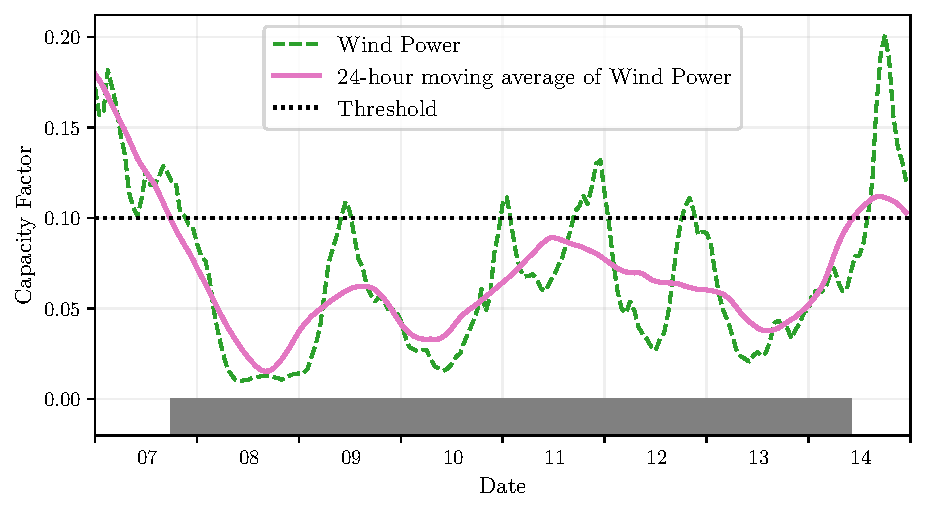
\includegraphics[width=\textwidth]{droughts_methodology.pdf}
	\caption{Wind time series of CF (green) and its 24-hour moving average (pink) from the 7th to the 15th of July 2021. The black dashed line indicates the CF threshold. The grey bar shows the period identified as a wind drought under our definition}
	\label{fig:find_res_droughts}
\end{figure}

The moving average approach smooths out short-term fluctuations, so that brief periods above the threshold do not interrupt an otherwise continuous low-CF period (Fig.~\ref{fig:find_res_droughts}). This means that a single hour above the threshold does not "break" a \DIFaddbegin \DIFadd{RES }\DIFaddend drought event if it is surrounded by prolonged low-generation hours. As a result, fewer but longer-lasting \DIFaddbegin \DIFadd{RES }\DIFaddend drought events are identified, which may better reflect \DIFdelbegin \DIFdel{real-world }\DIFdelend \DIFaddbegin \DIFadd{actual }\DIFaddend conditions where energy supply constraints persist over extended periods.

\section{Results}
\DIFdelbegin %DIFDELCMD < \label{sec:Results}
%DIFDELCMD < %%%
\DIFdelend \DIFaddbegin \label{sec:results}
\DIFaddend 

\subsection{Verification}
\label{sec:verification}

The accuracy of the datasets used in this study was verified, before continuing to the analysis of RES droughts. For the verification process, time-varying values of installed capacity were used to account for changes in RES development over the verification period. This step allowed us to assess how well the datasets represent the production of renewable energy by comparing them against observed data. \DIFaddbegin \DIFadd{This validation step evaluates how well the datasets represent actual renewable energy production by comparing them against observed data. The overall statistical distribution of CF values for wind (2014–2023) and solar PV (2023) is presented in the violin plots in Fig.~\ref{fig:violin_plots}. These plots illustrate the density of CF values for each dataset, highlighting their differences and alignment with observations. The results indicate that ATL aligns more closely with OBS for wind, while all datasets exhibit similar distributions for solar PV.
}

\begin{figure}[ht!]
	\centering
	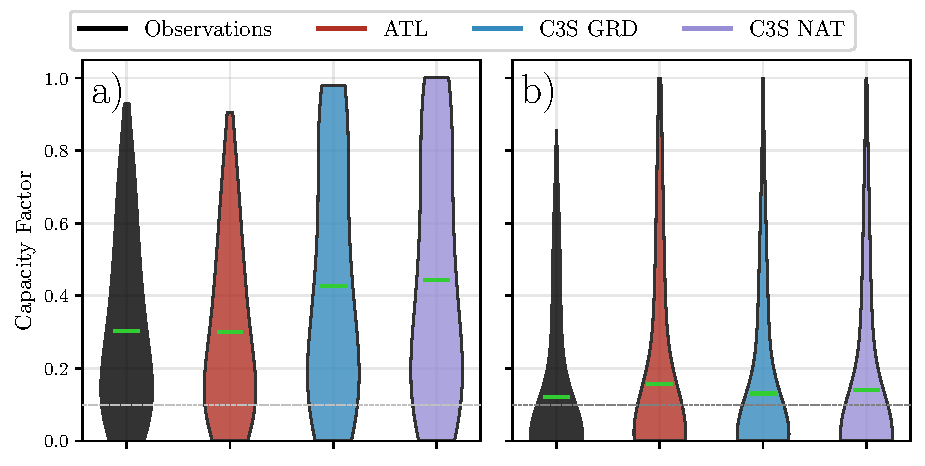
\includegraphics[width=\textwidth]{violin_plots_verification.pdf}
	\caption{\DIFaddFL{Violin plots of CF distributions for a)  wind and b) solar PV for the Observations (grey) and the three datasets: ATL (red), C3S~GRD (blue), and C3S~NAT (purple). The black dot shows the median values, while the black vertical lines represent the first and third quartiles. The black dashed line indicates the threshold of 0.1 used in the study to identify RES droughts}}
	\label{fig:violin_plots}
\end{figure}
\DIFaddend 

\subsubsection{Wind Energy}
\label{sec:wind_verification}

The \DIFdelbegin \DIFdel{C3S-E }\DIFdelend \DIFaddbegin \DIFadd{C3S }\DIFaddend datasets use the Vestas V136/3450 wind turbine power curve \DIFdelbegin \DIFdel{, }\DIFdelend (Fig.~\ref{fig:power_curve}a). The Atlite model allows the user to specify the power curve. We considered the 121 power curves available for download from Renewables.ninja~\citep{staffell2016wake}. For each power curve, Renewables.ninja also provides four associated smoothed power curves. The smoothing is done using a Gaussian filter with different standard deviations that depend on the wind speed. A separate wind CF time series for Ireland was generated for each of the wind turbine power curves and smoothing levels.

The performance of each CF time series is then assessed based on four skill scores: correlation coefficient (CC), root mean square error (RMSE), mean bias error (MBE), and the percentage of overlap. The percentage of overlap quantifies the similarity between the observed and modelled distributions. It is a positively oriented skill score, where 100\% shows full agreement between the two distributions, and 0\% indicates no overlap. The histograms of hourly CF values for the most recent decade (2014-2023) are used to calculate this skill score.

\begin{figure}[!ht]
	\centering
	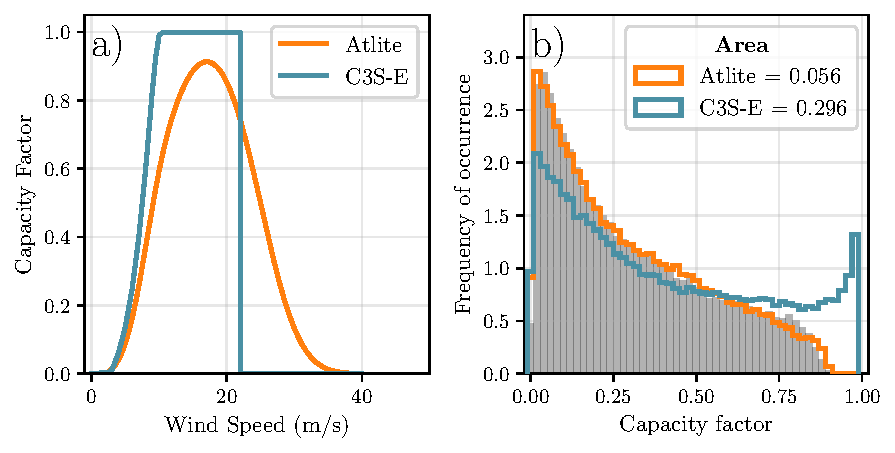
\includegraphics[width=\textwidth]{verification_power_curve.pdf}
	\caption{a) Power curves of the Enercon E112.4500 with a 0.3w smoothing filter used by \DIFdelbeginFL \DIFdelFL{Atlite }\DIFdelendFL \DIFaddbeginFL \DIFaddFL{the ATL dataset }\DIFaddendFL (orange) and the Vestas V136/3450 used by \DIFdelbeginFL \DIFdelFL{C3S-E }\DIFdelendFL \DIFaddbeginFL \DIFaddFL{the two C3S datasets }\DIFaddendFL (blue) b) Histograms of wind CF for Ireland \DIFdelbeginFL \DIFdelFL{from Atlite }\DIFdelendFL \DIFaddbeginFL \DIFaddFL{for the ATL dataset }\DIFaddendFL (orange), \DIFdelbeginFL \DIFdelFL{C3S-E }\DIFdelendFL \DIFaddbeginFL \DIFaddFL{the C3S datasets }\DIFaddendFL (blue) and Observed (shaded)}
	\label{fig:power_curve}
\end{figure}

Based on these metrics, the most representative power curve for Ireland is the Enercon E112.4500 power curve with the $0.3w$ smoothing filter. The smoothing of the wind turbine power curve represents losses associated with each turbine, as well as losses such as wake effects between turbines, which are important when modelling wind energy on larger spatial scales. The histogram in Fig.~\ref{fig:power_curve}b shows that the \DIFdelbegin \DIFdel{C3S-E }\DIFdelend \DIFaddbegin \DIFadd{C3SE }\DIFaddend power curve tends to underestimate low CF values and overestimate higher ones, whereas the smoothed \DIFdelbegin \DIFdel{Atlite }\DIFdelend \DIFaddbegin \DIFadd{ATL }\DIFaddend power curve more closely follows the observed wind availability data. This is further supported by the percentage of overlap which is higher for \DIFdelbegin \DIFdel{Atlite }\DIFdelend \DIFaddbegin \DIFadd{ATL }\DIFaddend (97.2\%) than for \DIFdelbegin \DIFdel{C3S-E }\DIFdelend \DIFaddbegin \DIFadd{C3SE }\DIFaddend (83.2\%), indicating better agreement with observed data.

\begin{figure}[!ht]
	\centering
	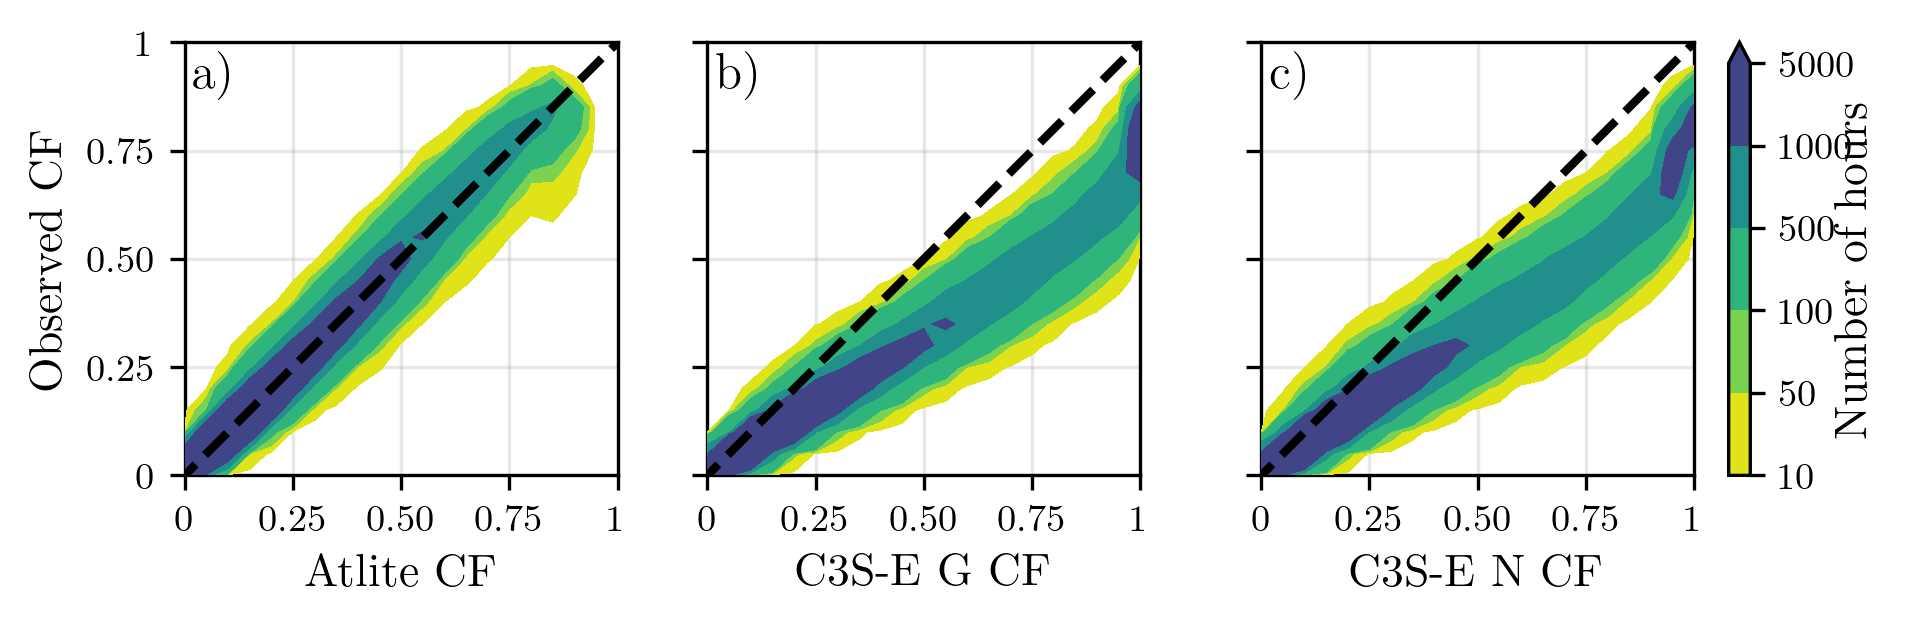
\includegraphics[width=\textwidth]{verification_wind_contour.png}
	\caption{Wind CF density plot of the observed CF (vertical axes) and modelled (horizontal axes) CF data for the a) \DIFdelbeginFL \DIFdelFL{Atlite}\DIFdelendFL \DIFaddbeginFL \DIFaddFL{ATL}\DIFaddendFL , b) \DIFdelbeginFL \DIFdelFL{C3S-E G }\DIFdelendFL \DIFaddbeginFL \DIFaddFL{C3S~GRD }\DIFaddendFL and c) \DIFdelbeginFL \DIFdelFL{C3S-E N models}\DIFdelendFL \DIFaddbeginFL \DIFaddFL{C3S~NAT datasets}\DIFaddendFL }
	\label{fig:wind_verification_contour}
\end{figure}

The effect of the difference between the power curves is also visible in Fig.~\ref{fig:wind_verification_contour}, which shows a density plot of wind CF values. The two \DIFdelbegin \DIFdel{C3S-E }\DIFdelend \DIFaddbegin \DIFadd{C3S }\DIFaddend datasets are shown to overestimate the observed CF, whereas the \DIFdelbegin \DIFdel{Atlite model }\DIFdelend \DIFaddbegin \DIFadd{ATL dataset }\DIFaddend is in good agreement with the observed data. The skill scores presented in Table~\ref{tab:wind_skill_scores} show that \DIFdelbegin \DIFdel{Atlite }\DIFdelend \DIFaddbegin \DIFadd{ATL }\DIFaddend performs better than the \DIFdelbegin \DIFdel{C3S-E }\DIFdelend \DIFaddbegin \DIFadd{two C3S }\DIFaddend datasets for all of the skill scores. 

\begin{table}[!ht]
	\centering
	\begin{tabular}{l|lll|}
		\cline{2-4}
		& \textbf{\DIFdelbeginFL \DIFdelFL{Atlite}\DIFdelendFL \DIFaddbeginFL \DIFaddFL{ATL}\DIFaddendFL } & \textbf{\DIFdelbeginFL \DIFdelFL{C3S-E G}\DIFdelendFL \DIFaddbeginFL \DIFaddFL{C3S~GRD}\DIFaddendFL } & \textbf{\DIFdelbeginFL \DIFdelFL{C3S-E N}\DIFdelendFL \DIFaddbeginFL \DIFaddFL{C3S~NAT}\DIFaddendFL } \\ \hline
		\multicolumn{1}{|l|}{\textbf{CC}}   & 0.981           & 0.972            & 0.970            \\ \hline
		\multicolumn{1}{|l|}{\textbf{RMSE}} & 0.045           & 0.177            & 0.162            \\ \hline
		\multicolumn{1}{|l|}{\textbf{MBE}}   & -0.003          & 0.137            & 0.121            \\ \hline
	\end{tabular}
	\caption{Skill scores for wind power for the three datasets compared to observed data}
	\label{tab:wind_skill_scores}
\end{table}

Fig.~\ref{fig:bar_number_events_verification_wind} shows the average annual number of wind drought events during the 2014 to 2023 validation period. The figure reveals that \DIFdelbegin \DIFdel{Atlite }\DIFdelend \DIFaddbegin \DIFadd{ATL }\DIFaddend presents the best overall agreement with the observed frequency and duration of wind drought events. This pattern is particularly evident for shorter-duration events, which are the most frequent.

\begin{figure}[!ht]
	\centering
	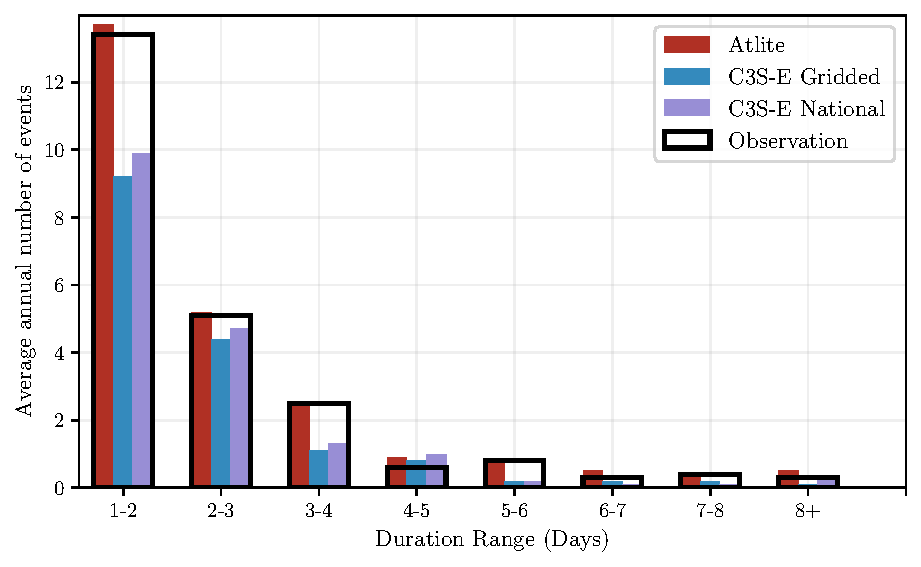
\includegraphics[width=\textwidth]{verification_wind_number_events.pdf}
	\caption{Average annual number of wind drought events for \DIFdelbeginFL \DIFdelFL{Atlite }\DIFdelendFL \DIFaddbeginFL \DIFaddFL{ATL }\DIFaddendFL (red), \DIFdelbeginFL \DIFdelFL{C3S-E G }\DIFdelendFL \DIFaddbeginFL \DIFaddFL{C3S~GRD }\DIFaddendFL (blue), \DIFdelbeginFL \DIFdelFL{C3S-E N }\DIFdelendFL \DIFaddbeginFL \DIFaddFL{C3S~NAT }\DIFaddendFL (purple), and the observed data (black outline). The wind droughts are identified from 2014 to 2023, considering the actual capacity of the system at any given time}
	\label{fig:bar_number_events_verification_wind}
\end{figure}

\DIFaddbegin \DIFadd{This verification for wind generation data highlights the importance of selecting a representative wind turbine power curve for the region being analysed. The ATL dataset, which uses a representative wind turbine power curve, is skilled at reproducing wind CF and RES droughts over Ireland. On the other hand, the power curve used for both C3S~GRD and C3S~NAT is not representative for Ireland, as it severely overestimates generation, underestimating the occurrence of RES droughts. This highlights a problem with using generalised datasets for analysing RES droughts: biases severely affect their ability to accurately reproduce RES drought events. The skill scores for the three datasets (Tab.~\ref{tab:wind_skill_scores}) show only a small difference in their ability to reproduce the changes in CF, as seen by their similar CC scores. However, their ability to reproduce the actual CF values is much lower than that of ATL, with RMSE scores almost four times bigger for the two C3S datasets. There is a clear bias towards an overestimation of CF, seen in the MBE values, which leads to the underestimation of RES droughts. This highlights the need to use regionally verified datasets to assess RES droughts.
}

\DIFaddend \subsubsection{\DIFaddbegin \DIFadd{Solar }\DIFaddend PV Energy}
\label{sec:pv_verification}

The Atlite model allows the user to select certain PV panel characteristics. In this study, the three PV panel types available in the Atlite model were considered (CSi, CdTe, Kaneka). Following the same methodology as in the previous section, the three available models were compared using four skill scores (CC, RMSE, MBE, and the percentage of overlap). Based on the best-performing metrics, the \DIFdelbegin \DIFdel{Breyer }\DIFdelend \DIFaddbegin \DIFadd{Beyer }\DIFaddend PV panel model was selected\DIFaddbegin \DIFadd{~}\DIFaddend \citep{beyer2004pv}, using the Kaneka Hybrid panel option. For all \DIFaddbegin \DIFadd{solar }\DIFaddend PV farm locations, the azimuth angle is fixed at 180\textdegree (due south), and the optimal tilt angle option is applied. 

The \DIFaddbegin \DIFadd{solar }\DIFaddend PV installed capacity available on the spreadsheets from EirGrid represents the Maximum Export Capacity (MEC) and does not accurately reflect the installed \DIFaddbegin \DIFadd{solar }\DIFaddend PV capacity. To enable actual \DIFaddbegin \DIFadd{solar }\DIFaddend PV generation potential to be modelled correctly, installed capacities were set at 1.4 times the MEC values. This scaling factor was estimated by analysing proprietary data from individual \DIFaddbegin \DIFadd{solar }\DIFaddend PV farms provided by EirGrid, which showed that, on average, assuming that the installed capacities of farms exceed their MEC values by 40\% yields the best agreement with the observed availability.

\begin{figure}[h!]
	\centering
	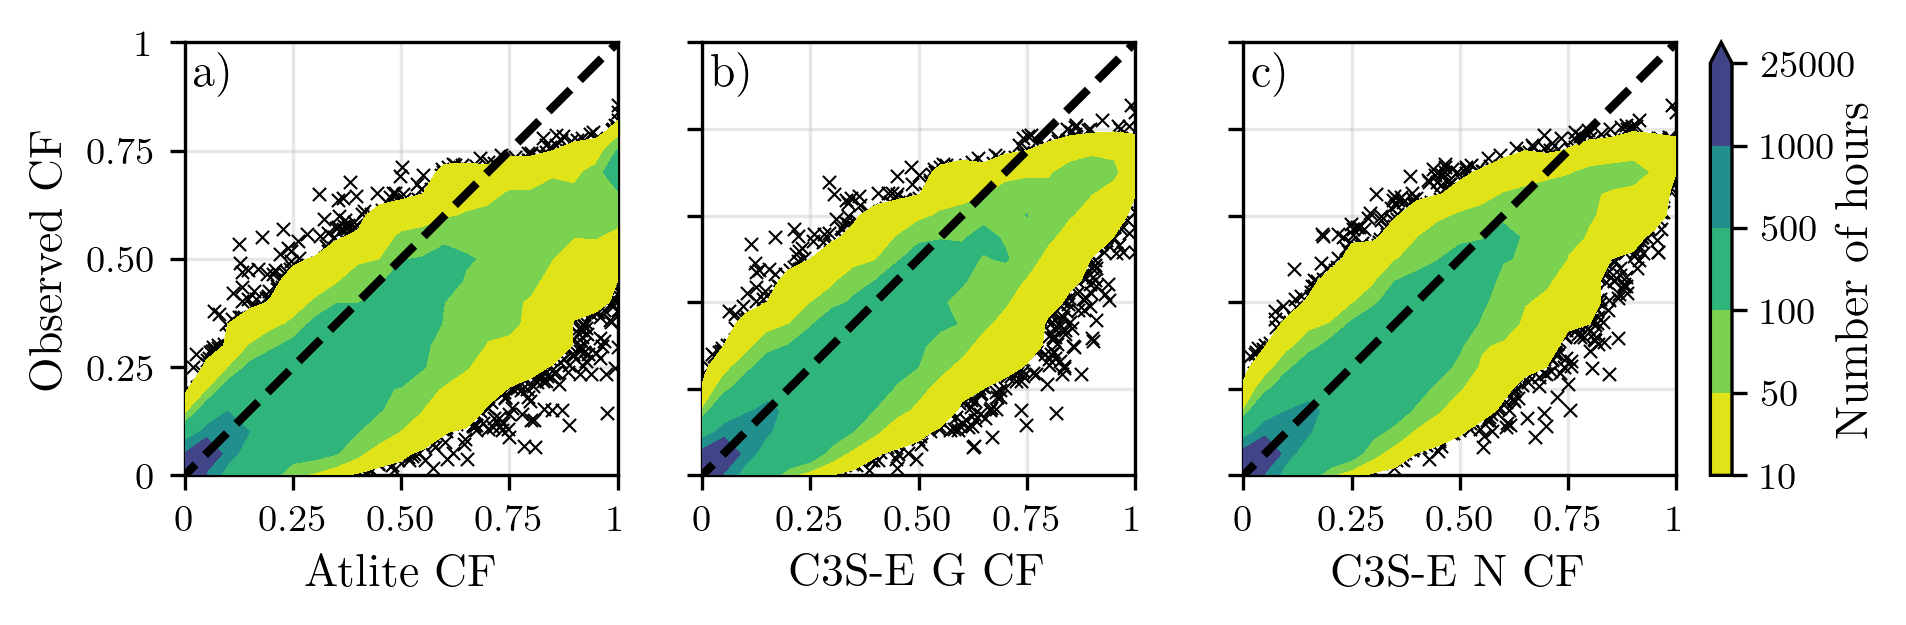
\includegraphics[width=\textwidth]{verification_pv_contour.png}
	\caption{\DIFaddbeginFL \DIFaddFL{Solar }\DIFaddendFL PV CF density plot of the observed (vertical axes) and modelled (horizontal axes) CF series for the a) \DIFdelbeginFL \DIFdelFL{Atlite}\DIFdelendFL \DIFaddbeginFL \DIFaddFL{ATL}\DIFaddendFL , b) \DIFdelbeginFL \DIFdelFL{C3S-E G }\DIFdelendFL \DIFaddbeginFL \DIFaddFL{C3S~GRD }\DIFaddendFL and c) \DIFdelbeginFL \DIFdelFL{C3S-E N models}\DIFdelendFL \DIFaddbeginFL \DIFaddFL{C3S~NAT datasets}\DIFaddendFL }	
	\label{fig:solar_verification_contour}
\end{figure}

\DIFdelbegin \DIFdel{Figure }\DIFdelend \DIFaddbegin \DIFadd{Fig.~}\DIFaddend \ref{fig:solar_verification_contour} shows that the three datasets have a similar tendency to overestimate the CF compared to the observed values, especially for high CF values. The skill scores presented in Table~\ref{tab:pv_skill_scores} indicate that \DIFdelbegin \DIFdel{C3S-E~G performs best overall, with the lowest RMSE and a high correlation coefficient, suggesting a closer match to observed data. All models show a slight positive bias, with Atlite exhibiting a slightly lower correlation and higher RMSE}\DIFdelend \DIFaddbegin \DIFadd{C3S~GRD and C3S~NAT perform better than ATL for solar PV CF, with lower RMSE and MBE, and higher CC scores. This may be due to the statistical approach taken by C3SE for the orientation of the PV panels}\DIFaddend .

\begin{table}[!ht]
	\centering
	\begin{tabular}{l|lll|}
		\cline{2-4}
		& \textbf{\DIFdelbeginFL \DIFdelFL{Atlite}\DIFdelendFL \DIFaddbeginFL \DIFaddFL{ATL}\DIFaddendFL } & \textbf{\DIFdelbeginFL \DIFdelFL{C3S-E G}\DIFdelendFL \DIFaddbeginFL \DIFaddFL{C3S~GRD}\DIFaddendFL } & \textbf{\DIFdelbeginFL \DIFdelFL{C3S-E N}\DIFdelendFL \DIFaddbeginFL \DIFaddFL{C3S~NAT}\DIFaddendFL } \\ \hline
		\multicolumn{1}{|l|}{\textbf{CC}}   & 0.921           & 0.931            & 0.931            \\ \hline
		\multicolumn{1}{|l|}{\textbf{RMSE}} & 0.119           & 0.090            & 0.113            \\ \hline
		\multicolumn{1}{|l|}{\textbf{MBE}}   & 0.046           & 0.027           & 0.021           \\ \hline
	\end{tabular}
	\caption{Skill scores for \DIFaddbeginFL \DIFaddFL{solar }\DIFaddendFL PV CF for the three datasets compared to observed data}
	\label{tab:pv_skill_scores}
\end{table}

Fig.~\ref{fig:bar_number_events_verification_pv} shows the number of \DIFaddbegin \DIFadd{solar }\DIFaddend PV drought events during the 2023 validation period across different duration ranges. The figure reveals partial agreement between the three datasets and the observed data, with consistent results noticed for duration ranges of 1-2, 3-4, 7-8, and 8+ days. However, discrepancies appear in the other ranges, where the \DIFdelbegin \DIFdel{models }\DIFdelend \DIFaddbegin \DIFadd{datasets }\DIFaddend diverge from the observed data. The main challenge in validating \DIFaddbegin \DIFadd{solar }\DIFaddend PV data stems from the recent installation of a large share of Ireland’s \DIFaddbegin \DIFadd{solar }\DIFaddend PV capacity, with over 65\% of the total \DIFaddbegin \DIFadd{solar }\DIFaddend PV capacity installed in 2023. This results in uncertainties in \DIFaddbegin \DIFadd{solar }\DIFaddend PV generation data and the actual generating capacity in the first few months after each farm is connected. \DIFdelbegin %DIFDELCMD < 

%DIFDELCMD < %%%
\DIFdel{As the goal of this analysis is to assess the combination of wind and PV generation, the complementary nature of these energy sources mitigates the limitations in PV-only results}\DIFdelend \DIFaddbegin \DIFadd{Overall, C3S~GRD performs slightly better than the other datasets in reproducing observed solar PV drought events}\DIFaddend .

\begin{figure}[!ht]
	\centering
	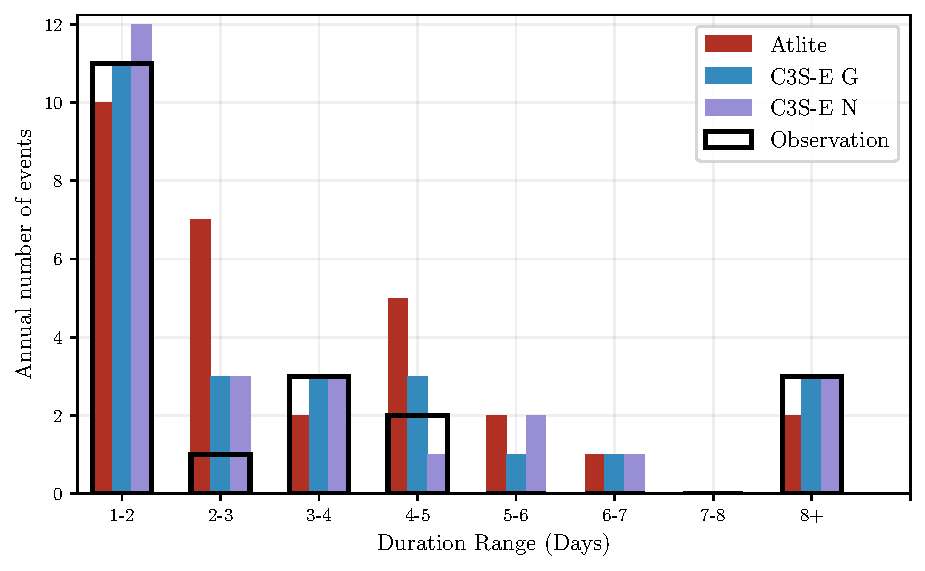
\includegraphics[width=\textwidth]{verification_pv_number_events.pdf}
	\caption{Number of \DIFaddbeginFL \DIFaddFL{solar }\DIFaddendFL PV drought events for \DIFdelbeginFL \DIFdelFL{Atlite }\DIFdelendFL \DIFaddbeginFL \DIFaddFL{ATL }\DIFaddendFL (red), \DIFdelbeginFL \DIFdelFL{C3S-E G }\DIFdelendFL \DIFaddbeginFL \DIFaddFL{C3S~GRD }\DIFaddendFL (blue), and \DIFdelbeginFL \DIFdelFL{C3S-E N }\DIFdelendFL \DIFaddbeginFL \DIFaddFL{C3S~NAT }\DIFaddendFL (purple) and the observed data (black outline). The \DIFaddbeginFL \DIFaddFL{solar }\DIFaddendFL PV droughts are identified for 2023, considering the actual capacity of the system at any given time}
	\label{fig:bar_number_events_verification_pv}
\end{figure}

\subsection{Analysis}
\DIFdelbegin %DIFDELCMD < \label{sec:Analysis}
%DIFDELCMD < %%%
\DIFdelend \DIFaddbegin \label{sec:analysis}
\DIFaddend 

In this section, RES \DIFaddbegin \DIFadd{droughts are analysed by calculating the frequency and duration of RES drought events, the return periods for different RES drought durations, and the seasonality of RES drought events. Understanding the characteristics and timing of RES drought events enables system operators to optimally plan for reserve capacity requirements, ensuring grid stability and security of supply. Results are presented for the three datasets, allowing their differences on the characterisation of RES droughts to be clearly identified.
}

\DIFadd{RES }\DIFaddend drought events are evaluated under two different scenarios with fixed installed capacities: the 91W-9PV scenario, with 5.9 GW of wind capacity and 0.6 GW of \DIFaddbegin \DIFadd{solar }\DIFaddend PV capacity; and the 57W-43PV scenario, where wind capacity comprises 11.45 GW and \DIFaddbegin \DIFadd{solar }\DIFaddend PV capacity increases to 8.6 GW. Both scenarios were driven by 45 years of ERA5 data. Using the RES drought identification process described in Section~\ref{sec:res_drought}, wind and \DIFaddbegin \DIFadd{solar }\DIFaddend PV droughts are first analysed separately before presenting the results for combined (wind + \DIFaddbegin \DIFadd{solar }\DIFaddend PV) RES droughts under both scenarios.

\subsubsection{Annual Number of RES Droughts}

The first part of the analysis examines the annual number of RES drought events\DIFdelbegin \DIFdel{across the three datasets}\DIFdelend . When only wind energy is considered (Fig.~\ref{fig:boxplot_number_events}a), the number of \DIFaddbegin \DIFadd{RES drought }\DIFaddend events decreases as the duration range increases, with very few events lasting more than seven days. In \DIFdelbegin \DIFdel{the case of only }\DIFdelend \DIFaddbegin \DIFadd{contrast, for solar }\DIFaddend PV energy (Fig.~\ref{fig:boxplot_number_events}b), \DIFdelbegin \DIFdel{the number of events also declines as the duration range extends }\DIFdelend \DIFaddbegin \DIFadd{RES drought frequency declines }\DIFaddend from one to eight days \DIFdelbegin \DIFdel{, followed by a slight increase }\DIFdelend \DIFaddbegin \DIFadd{and then slightly increases }\DIFaddend for longer durations. This \DIFdelbegin \DIFdel{increase occurs because Ireland, being located above the 50\textdegree~parallel, experiences reduced sunlight during the winter months. From }\DIFdelend \DIFaddbegin \DIFadd{behaviour is attributable to Ireland's high-latitude location, where reduced sunlight in winter (from }\DIFaddend November to March\DIFdelbegin \DIFdel{, PV output often remains consistently low , leading to extended periods where generation stays below the CF threshold}\DIFdelend \DIFaddbegin \DIFadd{) leads to consistently low solar PV output}\DIFaddend .

\DIFdelbegin \DIFdel{When comparing wind and PV results (Fig.~\ref{fig:boxplot_number_events}a~\&~b), }\DIFdelend \DIFaddbegin \DIFadd{Moreover, the comparison between wind and solar PV results indicates that }\DIFaddend the median, first, and third quartiles for \DIFaddbegin \DIFadd{solar }\DIFaddend PV are consistently higher than or equal to those for wind\DIFdelbegin \DIFdel{, across all duration ranges and datasets}\DIFdelend . This is \DIFdelbegin \DIFdel{due to the typically lower CF of PV power compared to wind power, especially in a region such as Ireland where solar potential is limited. }\DIFdelend \DIFaddbegin \DIFadd{expected, given that solar }\DIFaddend PV generation is \DIFdelbegin \DIFdel{also }\DIFdelend \DIFaddbegin \DIFadd{inherently lower, }\DIFaddend zero at night\DIFdelbegin \DIFdel{and constrained by the daily solar cycle, leading to a naturally higher frequency of drought events in PV compared to wind. }%DIFDELCMD < 

%DIFDELCMD < %%%
\DIFdel{Fig.~\ref{fig:boxplot_number_events}c~\&~d show the combination of wind and PV under the two capacity scenarios. In the }\DIFdelend \DIFaddbegin \DIFadd{, and limited by the solar cycle. When wind and solar PV are combined under the }\DIFaddend 91W-9PV scenario (Fig.~\ref{fig:boxplot_number_events}c), the \DIFdelbegin \DIFdel{identified RES droughts closely match those for }\DIFdelend \DIFaddbegin \DIFadd{results closely mirror those of }\DIFaddend wind alone, \DIFdelbegin \DIFdel{which is expected }\DIFdelend due to the dominance of \DIFdelbegin \DIFdel{installed wind capacity. In contrast, }\DIFdelend \DIFaddbegin \DIFadd{wind power in the current energy mix. However, in }\DIFaddend the 57W-43PV scenario (Fig.~\ref{fig:boxplot_number_events}d)\DIFdelbegin \DIFdel{shows a clear reduction in the number of drought events }\DIFdelend \DIFaddbegin \DIFadd{, a marked reduction in RES drought events is observed }\DIFaddend across all datasets\DIFdelbegin \DIFdel{and durations}\DIFdelend , with a decrease of the total number of events of 56\% for \DIFdelbegin \DIFdel{Atlite}\DIFdelend \DIFaddbegin \DIFadd{ATL}\DIFaddend , 52\% for \DIFdelbegin \DIFdel{C3S-E G}\DIFdelend \DIFaddbegin \DIFadd{C3S~GRD}\DIFaddend , and 50\% for \DIFdelbegin \DIFdel{C3S-E N. This reduction is attributed to the anti-correlation between wind and PV generation}\DIFdelend \DIFaddbegin \DIFadd{C3S~NAT, demonstrating the beneficial effects of a more equal share of wind and solar PV capacity}\DIFaddend .

The \DIFdelbegin \DIFdel{median, first, and third quartiles for the Atlite datasetare consistently greater than or equal to those of the other two datasets, regardless of the duration range or type of renewable energy considered. This difference arises from the }\DIFdelend \DIFaddbegin \DIFadd{consistently higher RES drought counts reported by the ATL dataset, compared to the C3S datasets, underscore the importance of }\DIFaddend wind turbine power curve \DIFdelbegin \DIFdel{model used in the C3S-E datasets , which tends to overestimate the wind CF (Fig.~\ref{fig:wind_verification_contour}). As a result, the overall number of RES droughts is underestimated in the C3S-E datasets compared to Atlite}\DIFdelend \DIFaddbegin \DIFadd{representation when quantifying RES droughts. Whereas the three datasets agree on the overall effect of balancing the share of wind and solar PV generation, they differ at a quantitative level, which has crucial implications for energy planning}\DIFaddend .

\begin{figure}[!ht]
	\centering
	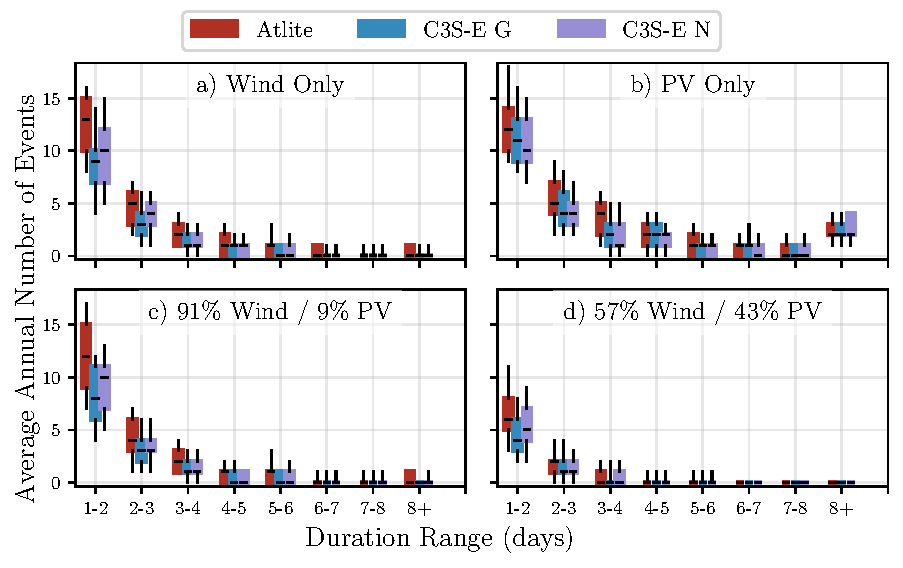
\includegraphics[width=\textwidth]{droughts_number_events.pdf}
	\caption{Average annual number of RES droughts (from 1979 to 2023) for a)~Wind, b)~\DIFaddbeginFL \DIFaddFL{solar }\DIFaddendFL PV, c)~91W-9PV and d)~57W-43PV for \DIFdelbeginFL \DIFdelFL{Atlite }\DIFdelendFL \DIFaddbeginFL \DIFaddFL{ATL }\DIFaddendFL (red), \DIFdelbeginFL \DIFdelFL{C3S-E G }\DIFdelendFL \DIFaddbeginFL \DIFaddFL{C3S~GRD }\DIFaddendFL (blue), and \DIFdelbeginFL \DIFdelFL{C3S-E N }\DIFdelendFL \DIFaddbeginFL \DIFaddFL{C3S~NAT }\DIFaddendFL (purple). The x-axis represents duration ranges in days (lower bound included), while the y-axis indicates the annual number of events. The boxes display the first and third quartiles and the median is marked by a black line. The whiskers indicate the 5th and 95th percentiles}
	\label{fig:boxplot_number_events}	
\end{figure}

\subsubsection{Return Periods of RES Drought Duration}

\DIFdelbegin \DIFdel{The }\DIFdelend RES drought events identified over the 45-year period were used to calculate the return periods for different RES drought durations. A return period is the estimated average time interval between events of a specified duration \DIFdelbegin \DIFdel{or intensity }\DIFdelend (not to be confused with the frequency of their occurrence within a fixed time frame). Fig.~\ref{fig:return_periods} \DIFdelbegin \DIFdel{illustrates }\DIFdelend \DIFaddbegin \DIFadd{shows }\DIFaddend the return periods for \DIFdelbegin \DIFdel{varying }\DIFdelend \DIFaddbegin \DIFadd{different }\DIFaddend RES drought durations, \DIFdelbegin \DIFdel{highlighting how often different drought lengths are likely to occur across the datasets. This analysis provides insight into the frequency and likelihood of prolonged low-generation periods , which is crucialfor evaluating the potential impact of RES droughts on energy reliability and }\DIFdelend \DIFaddbegin \DIFadd{which can be used to capture the most extreme events affecting the system. Understanding their return periods is crucial, as extreme yet rare RES droughts pose the toughest challenge to energy security by placing significant strain on the conventional backup sources necessary to maintain }\DIFaddend security of supply \DIFaddbegin \DIFadd{during these events}\DIFaddend .

The duration of wind droughts (Fig.~\ref{fig:return_periods}a) increases in a log-linear fashion across the three datasets. The log-linear trend indicates a predictable relationship between \DIFaddbegin \DIFadd{wind }\DIFaddend drought duration and occurrence, with longer wind droughts becoming exponentially less likely as duration increases. \DIFdelbegin %DIFDELCMD < 

%DIFDELCMD < %%%
\DIFdelend In the case of \DIFaddbegin \DIFadd{solar }\DIFaddend PV droughts (Fig.~\ref{fig:return_periods}b), Atlite behaves differently than the two \DIFdelbegin \DIFdel{C3S-E }\DIFdelend \DIFaddbegin \DIFadd{C3S }\DIFaddend datasets. The \DIFdelbegin \DIFdel{Atlite results }\DIFdelend \DIFaddbegin \DIFadd{ATL dataset }\DIFaddend show a generally log-linear increase. For \DIFdelbegin \DIFdel{C3S-E G and C3S-E N}\DIFdelend \DIFaddbegin \DIFadd{C3S~GRD and C3S~NAT}\DIFaddend , the duration of PV droughts increases in a log-linear pattern for events lasting less than 16 days. Beyond this duration, there is a sharp rise in \DIFaddbegin \DIFadd{solar PV }\DIFaddend drought duration for events up to a one-year return period. This sudden increase again reflects the impact of extended periods of low PV generation during winter in Ireland. \DIFdelbegin %DIFDELCMD < 

%DIFDELCMD < %%%
\DIFdelend The difference between \DIFdelbegin \DIFdel{Atlite and the C3S-E }\DIFdelend \DIFaddbegin \DIFadd{the ATL and the C3S }\DIFaddend results arises from differences in the datasets near the threshold of 0.1 CF. \DIFdelbegin \DIFdel{Atlite }\DIFdelend \DIFaddbegin \DIFadd{ATL }\DIFaddend remains slightly above the threshold more frequently during these conditions, leading to shorter, more fragmented \DIFaddbegin \DIFadd{RES }\DIFaddend drought events. In contrast, \DIFdelbegin \DIFdel{C3S-E G and C3S-E N }\DIFdelend \DIFaddbegin \DIFadd{C3S~GRD and C3S~NAT }\DIFaddend tend to fall below the threshold in similar conditions, resulting in longer continuous \DIFaddbegin \DIFadd{RES }\DIFaddend drought periods, especially during winter.

\DIFdelbegin \DIFdel{For }\DIFdelend \DIFaddbegin \DIFadd{Under }\DIFaddend the 91W-9PV scenario (Fig.~\ref{fig:return_periods}c), the \DIFaddbegin \DIFadd{combined RES drought }\DIFaddend return periods mirror those \DIFdelbegin \DIFdel{of Fig.~\ref{fig:return_periods}a, due to the low levels of installed PV capacity. In }\DIFdelend \DIFaddbegin \DIFadd{for wind alone, reflecting the dominance of wind in the current energy mix. In contrast, }\DIFaddend the 57W-43PV scenario (Fig.~\ref{fig:return_periods}d) \DIFdelbegin \DIFdel{, the return periods for RES droughts increase across all durations}\DIFdelend \DIFaddbegin \DIFadd{shows a dramatic reduction in RES drought durations, suggesting that a more balanced share of wind and solar PV capacity can substantially mitigate the frequency of prolonged RES drought events}\DIFaddend . For example, the return period for a five-day \DIFaddbegin \DIFadd{RES }\DIFaddend drought event (shown by the vertical dashed lines in Fig.~\ref{fig:return_periods}) \DIFdelbegin \DIFdel{extends }\DIFdelend \DIFaddbegin \DIFadd{increases }\DIFaddend from roughly six months for the 91W-9PV scenario, to four years for the 57W-43PV scenario in the \DIFdelbegin \DIFdel{Atlite }\DIFdelend \DIFaddbegin \DIFadd{ATL }\DIFaddend dataset, and from about fifteen months to around five years in the two \DIFdelbegin \DIFdel{C3S-E datasets. }\DIFdelend \DIFaddbegin \DIFadd{C3S datasets. This result indicates that the complementarity between wind and solar PV plays a crucial role in reducing the occurrence of RES drought events in a diversified energy portfolio.
}\DIFaddend 

\begin{figure}[!ht]
	\centering
	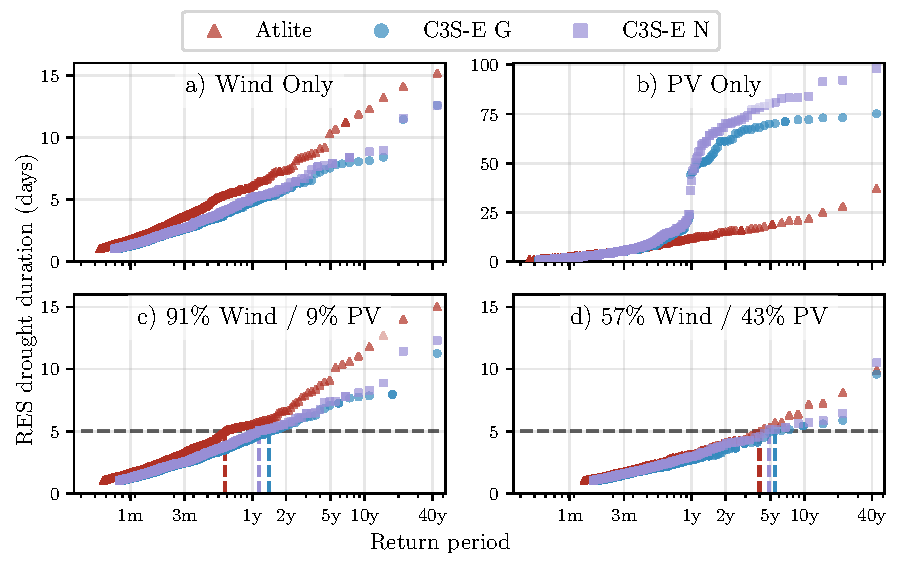
\includegraphics[width=\textwidth]{droughts_return_periods.pdf}
	\caption{Return periods of the duration of RES droughts  (from 1979 to 2023) for a)~Wind, b)~\DIFaddbeginFL \DIFaddFL{Solar }\DIFaddendFL PV, c)~91W-9PV and d)~57W-43PV for \DIFdelbeginFL \DIFdelFL{Atlite }\DIFdelendFL \DIFaddbeginFL \DIFaddFL{ATL }\DIFaddendFL (red triangle), \DIFdelbeginFL \DIFdelFL{C3S-E G }\DIFdelendFL \DIFaddbeginFL \DIFaddFL{C3S~GRD }\DIFaddendFL (blue circle), and \DIFdelbeginFL \DIFdelFL{C3S-E N }\DIFdelendFL \DIFaddbeginFL \DIFaddFL{C3S~NAT }\DIFaddendFL (purple square). The x-axis represents the return period time in a log-scale and the y-axis indicates the duration of RES drought associated with it. The horizontal dashed line marks the 5-day return period, with coloured vertical dashed marking its return period for each dataset}
	\label{fig:return_periods}
\end{figure}

Across Fig.~\ref{fig:return_periods}a, c, and \DIFdelbegin \DIFdel{, }\DIFdelend d, the return periods in the \DIFdelbegin \DIFdel{Atlite }\DIFdelend \DIFaddbegin \DIFadd{ATL }\DIFaddend dataset are consistently higher than those in the two \DIFdelbegin \DIFdel{C3S-E }\DIFdelend \DIFaddbegin \DIFadd{C3S }\DIFaddend datasets. For instance, in the 91W-9PV scenario (Fig.~\ref{fig:return_periods}c), an event with a one-year return period lasts six days in the \DIFdelbegin \DIFdel{Atlite }\DIFdelend \DIFaddbegin \DIFadd{ATL }\DIFaddend dataset, compared to only five days in the \DIFdelbegin \DIFdel{C3S-E }\DIFdelend \DIFaddbegin \DIFadd{C3S }\DIFaddend datasets. This difference underscores the importance of \DIFdelbegin \DIFdel{model }\DIFdelend \DIFaddbegin \DIFadd{dataset }\DIFaddend selection when quantifying RES droughts, as each \DIFdelbegin \DIFdel{model}\DIFdelend \DIFaddbegin \DIFadd{dataset}\DIFaddend ’s assumptions and parametrisations significantly influence \DIFdelbegin \DIFdel{drought }\DIFdelend \DIFaddbegin \DIFadd{RES droughts }\DIFaddend duration estimates. Additionally, in all four graphs, the similarity between results from the two \DIFdelbegin \DIFdel{C3S-E }\DIFdelend \DIFaddbegin \DIFadd{C3S }\DIFaddend datasets suggests that assumptions in the \DIFdelbegin \DIFdel{Atlite model—}\DIFdelend \DIFaddbegin \DIFadd{ATL dataset, }\DIFaddend such as wind turbine power curve selection and PV panel specifications\DIFdelbegin \DIFdel{—}\DIFdelend \DIFaddbegin \DIFadd{, }\DIFaddend have a greater impact on RES drought duration estimates than the precise geographic distribution of RES farms when studying the return periods of RES droughts.

\DIFaddbegin \DIFadd{The return periods calculated from the three datasets show large differences, in particular for the more extreme events with longer return periods. The C3S datasets produce shorter RES drought durations for these events, which would have the largest impact on the power system. This shows that system planning based on the wrong datasets could yield an underestimation of the duration of extreme RES droughts, potentially leading to shortages linked to undersized reserve capacity.
}

\DIFaddend \subsubsection{Seasonal Distribution of RES Droughts}

The \DIFdelbegin \DIFdel{seasonality }\DIFdelend \DIFaddbegin \DIFadd{seasonal analysis }\DIFaddend of RES droughts \DIFdelbegin \DIFdel{was analysed by comparing }\DIFdelend \DIFaddbegin \DIFadd{is based on }\DIFaddend the percentage of hours in each month classified as part of a RES drought \DIFaddbegin \DIFadd{event. Wind droughts tend to be more frequent during summer, whereas solar PV droughts are more common in winter due to reduced sunlight. By comparing these seasonal patterns across different datasets and energy scenarios, this study examines how dataset-specific assumptions and variations in capacity mix affect the overall characterisation of RES drought events}\DIFaddend .

For \DIFdelbegin \DIFdel{wind-dominated scenarios }\DIFdelend \DIFaddbegin \DIFadd{the wind-only scenario }\DIFaddend (Fig.~\ref{fig:res_droughts_seasonality}a\DIFdelbegin \DIFdel{~\&~c}\DIFdelend ), the \DIFdelbegin \DIFdel{percentage of hours that are part of a drought is higher in summer than in winter. In the Atlite dataset , for instance, an average of }\DIFdelend \DIFaddbegin \DIFadd{ATL dataset exhibits a pronounced seasonal pattern, with about }\DIFaddend 24\% of \DIFdelbegin \DIFdel{hours in summer (June-July-August) are identified as wind droughts , }\DIFdelend \DIFaddbegin \DIFadd{summer hours (June, July, August) identified as RES droughts }\DIFaddend compared to only 4\% in winter (\DIFdelbegin \DIFdel{December-January-February}\DIFdelend \DIFaddbegin \DIFadd{December, January, February}\DIFaddend ). This \DIFdelbegin \DIFdel{seasonal variation is less prominent for the two C3S-E datasetscompared to the Atlite one. This difference can be linked to the shape of the two power curves (Fig.~\ref{fig:power_curve}). CFs near or under }\DIFdelend \DIFaddbegin \DIFadd{strong seasonal signal is less evident in the C3S datasets, which suggests that the differences in the underlying wind power curves play a significant role. In ATL, CF near or below }\DIFaddend the 0.1 threshold \DIFdelbegin \DIFdel{occur at }\DIFdelend \DIFaddbegin \DIFadd{occurs at relatively }\DIFaddend higher wind speeds\DIFdelbegin \DIFdel{for the Atlite power curve than for the C3S-E one}\DIFdelend \DIFaddbegin \DIFadd{, resulting in a higher count of RES drought hours during the summer months}\DIFaddend . In contrast, \DIFdelbegin \DIFdel{the results for }\DIFdelend \DIFaddbegin \DIFadd{solar }\DIFaddend PV droughts (Fig.~\ref{fig:res_droughts_seasonality}b) \DIFdelbegin \DIFdel{show a higher percentage in winter, with PV droughts occurring }\DIFdelend \DIFaddbegin \DIFadd{display an opposite seasonal trend. Across all datasets, }\DIFaddend over 60\% of \DIFdelbegin \DIFdel{the time regardless of the dataset. 
The Atlite results show a }\DIFdelend \DIFaddbegin \DIFadd{winter hours are classified as solar PV droughts, reflecting the naturally low solar irradiance in Ireland during winter. 
}

\DIFadd{ATL tends to record a slightly }\DIFaddend higher percentage of \DIFdelbegin \DIFdel{PV }\DIFdelend \DIFaddbegin \DIFadd{RES }\DIFaddend drought hours for wind \DIFdelbegin \DIFdel{, and a slightly }\DIFdelend \DIFaddbegin \DIFadd{and a marginally }\DIFaddend lower percentage for \DIFdelbegin \DIFdel{PV, compared to the two C3S-E datasets. }%DIFDELCMD < 

%DIFDELCMD < \begin{figure}[!ht]
%DIFDELCMD < 	\centering
%DIFDELCMD < 	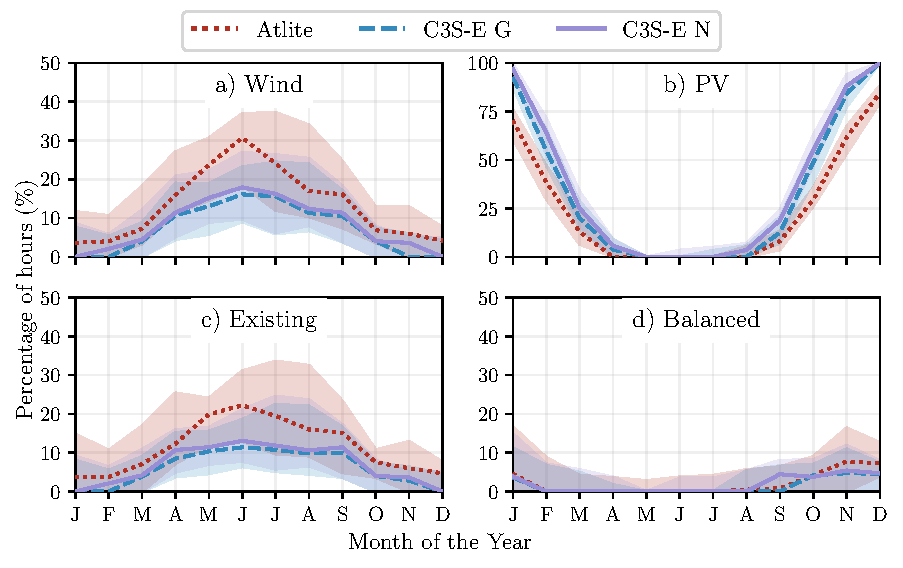
\includegraphics[width=\textwidth]{droughts_seasonality.pdf}
%DIFDELCMD < 	%%%
%DIFDELCMD < \caption{%
{%DIFAUXCMD
\DIFdelFL{Percentage of hours in a month which are part of a RES drought (from 1979 to 2023) for a)~Wind, b)~PV, c)~91W-9PV and d)~57W-43PV for Atlite (red dotted), C3S-E G (blue dashed), and C3S-E N (purple solid). The x-axis represents the month of the year, and the y-axis indicates the percentage of hours. Lines correspond to the median values and the area between the first and third quartiles is shaded. Note the different y-axis scale for b).}}
	%DIFAUXCMD
%DIFDELCMD < \label{fig:res_droughts_seasonality}
%DIFDELCMD < \end{figure}
%DIFDELCMD < %%%
\DIFdelend \DIFaddbegin \DIFadd{solar PV relative to the C3S datasets. These differences highlight how dataset-specific assumptions, such as the treatment of wind turbine power curves and PV panel characteristics, influences the seasonal dynamics of RES droughts.
}\DIFaddend 

The 91W-9PV scenario (Fig.~\ref{fig:res_droughts_seasonality}c) shows patterns \DIFdelbegin \DIFdel{comparable }\DIFdelend \DIFaddbegin \DIFadd{similar }\DIFaddend to the ones for wind droughts (Fig.~\ref{fig:res_droughts_seasonality}a). However, in the 91W/9PV scenario, the number of hours classified as RES droughts in summer decreases slightly compared to the wind-only scenario. This reduction can be explained by the contribution of \DIFaddbegin \DIFadd{solar }\DIFaddend PV generation during the summer months in the 91W-9PV scenario, even though it constitutes only \DIFdelbegin \DIFdel{11}\DIFdelend \DIFaddbegin \DIFadd{9}\DIFaddend \% of total capacity. Since the number of RES drought hours for \DIFaddbegin \DIFadd{solar }\DIFaddend PV in summer is near zero, this small contribution has a noticeable impact on reducing overall \DIFaddbegin \DIFadd{RES }\DIFaddend drought hours. In the 57W-43PV scenario (Fig.~\ref{fig:res_droughts_seasonality}d), all three datasets show a reduction in monthly RES drought frequency. Annual reductions in median RES drought frequency are observed across the datasets, dropping from 14\% to 5\% for \DIFdelbegin \DIFdel{Atlite}\DIFdelend \DIFaddbegin \DIFadd{ATL}\DIFaddend , from 8\% to 3\% for \DIFdelbegin \DIFdel{C3S-E G}\DIFdelend \DIFaddbegin \DIFadd{C3S~GRD}\DIFaddend , and from 9\% to 4\% for \DIFdelbegin \DIFdel{C3S-E N}\DIFdelend \DIFaddbegin \DIFadd{C3S~NAT}\DIFaddend . The balanced mix of wind and \DIFaddbegin \DIFadd{solar }\DIFaddend PV power in this scenario reduces the seasonal signal overall and significantly decreases the percentage of RES drought hours in the summer.

\DIFdelbegin \section{\DIFdel{Discussion and Conclusions}}
%DIFAUXCMD
\addtocounter{section}{-1}%DIFAUXCMD
%DIFDELCMD < \label{sec:Conclusion}
%DIFDELCMD < %%%
\DIFdelend \DIFaddbegin \begin{figure}[!ht]
	\centering
	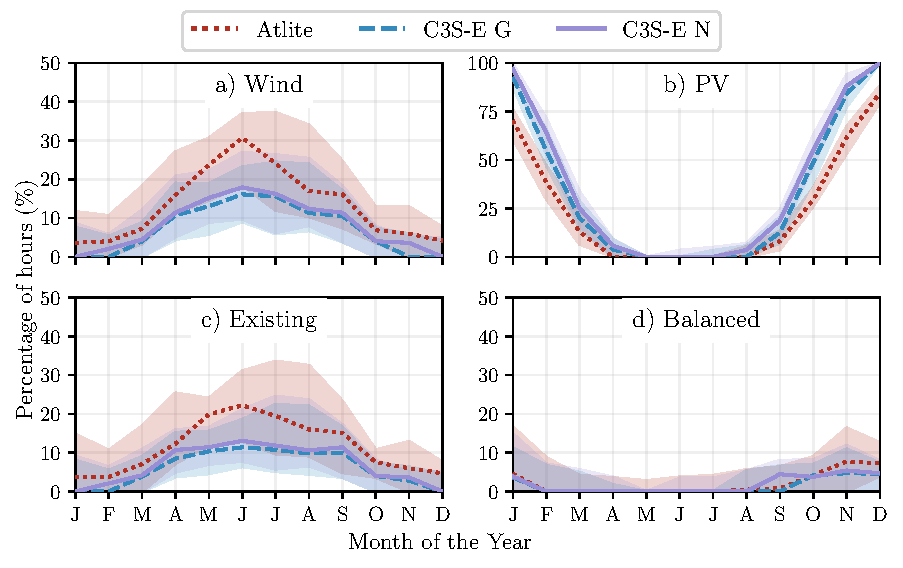
\includegraphics[width=\textwidth]{droughts_seasonality.pdf}
	\caption{\DIFaddFL{Percentage of hours in a month which are part of a RES drought (from 1979 to 2023) for a)~Wind, b)~Solar PV, c)~91W-9PV and d)~57W-43PV for ATL (red dotted), C3S~GRD (blue dashed), and C3S~NAT (purple solid). The x-axis represents the month of the year, and the y-axis indicates the percentage of hours. Lines correspond to the median values and the area between the first and third quartiles is shaded. Note the different y-axis scale for b).}}
	\label{fig:res_droughts_seasonality}
\end{figure}
\DIFaddend 

\DIFdelbegin \DIFdel{This study has investigated the ability of three RES models to represent RES droughts : Atlite, C3S-E G, and C3S-E N. One of the most evident differences is how each dataset incorporates the specific locations of RES farms. Both Atlite and C3S-E G consider the locations of wind and PV farms, which one would expect to result in a more accurate representation of RES generation. While this approach slightly improves PV models, our analysis indicates that for wind energy , the Atlite dataset performs better overall, especially in its close alignment with observed data for wind generation estimates.
This finding suggests that, although the inclusion of RES farm locations is beneficial, the accuracy of the }\DIFdelend \DIFaddbegin \DIFadd{The seasonal variations of RES droughts observed in this study have important implications for energy planning. Energy demand peaks in winter for Northern European countries, making the seasonality of }\DIFaddend RES \DIFdelbegin \DIFdel{model is more strongly influenced by underlying model assumptions, such as selecting an appropriate wind power curve.
}\DIFdelend \DIFaddbegin \DIFadd{droughts critical for the sizing of reserve capacity. Our results show that selecting the wrong dataset could severely underestimate RES droughts during winter months, thereby affecting the reliability of the energy system during critical periods. Additionally, the integration of large shares of solar PV in the system leads to a generalised reduction of RES droughts, yet winter months present a slight increase. The natural limitations of solar PV lead to inevitably higher reserve capacity needs during winter months as reliance on RES increases. These types of insights are essential to develop targeted strategies that enhance grid resilience and ensure a stable energy supply throughout the year.
}\DIFaddend 


\DIFdelbegin \DIFdel{Atlite shows the best alignment with observed data for wind generation. Differences between the models are smaller for PV, with C3S-G performing marginally better than the other two.
The results show that the two C3S-E datasets (C3S-E G and C3S-E N) consistently yield similar outcomes, indicating that their methodological differences have minimal impact in this case. This distinction is also evident in the analysis, where Atlite reports higher return periods and a greater number of RES droughts, especially in scenarios with a balanced share of RES . Again, the results from RES drought modelling rely more on the precision of the wind power curve and PV panel modelsthan on the specific locations of RES farms. Atlite’s superior performance highlights the importance of selecting validated models for assessing RES drought risks. This careful model selection can better quantify risks, support effective planning , and avoid the potential underestimation of capacity needs, which is essential for ensuring energy security }\DIFdelend \DIFaddbegin \section{\DIFadd{Conclusions}}
\label{sec:conclusions}

\DIFadd{This study aimed to answer two key questions: Do generic datasets have sufficient skill to reliably quantify RES drought events? How does the integration of solar PV into a predominantly wind-based system alter the characteristics of RES droughts? To address these questions, three datasets were compared: two derived from the European C3S-Energy dataset, and one developed by the authors. The datasets derived from C3S-Energy differ in their assumptions, one assumes a homogeneous distribution of wind and solar PV capacity across the region, while the other includes the actual locations of RES farms. The dataset developed by the authors uses a regionally validated model which accounts for farm locations and uses tailored wind and solar PV models selected to represent the actual generation.
}

\DIFadd{Our results demonstrate that datasets without regional validation misrepresent the frequency and duration of RES drought events due to their limited ability to reproduce the observations. The inclusion of wind and solar PV farm locations has limited impact on RES drought analysis compared to the choice of wind turbine power curves and solar PV models. Whereas all three datasets capture broad trends in the duration and seasonality of RES drought events, the actual number of events is consistently underestimated by the non-validated datasets. This effect becomes clearer for extreme events, as not using regionally validated datasets can yield an overestimation of the return periods of RES droughts. This can lead to insufficient reserve capacity planning and potential risks to grid stability and security of supply}\DIFaddend .

\DIFdelbegin \DIFdel{Looking at the 57W-43PV scenario, the analysis showed a significant improvement in the management of RES droughts due to the complementary nature }\DIFdelend \DIFaddbegin \DIFadd{The effect of the integration of solar PV capacity in a wind-dominated system on RES droughts has been explored. Our analysis has demonstrated that transitioning to a system with more equal amounts }\DIFaddend of wind and \DIFdelbegin \DIFdel{PV generation. Wind and PV together perform better in terms of reducing drought frequency and duration than either would individually, largely because of the seasonal anti-correlation between the two energy sources. This diversification reduces the seasonal impact on RES droughts, as PV generation peaks in the summer and wind generation is more consistent in winter. Ireland currently has a highly wind-dependent energy system, but with ambitious targets for PV installations in the coming years, the energy mix is expected to approach a balance between wind and PV capacity.
While this balanced approach offers a more stable and secure energy supply by mitigating RES drought risks, it is important to note that having similar wind and PV capacities may not optimise other aspects, such as annual energy production or meeting nighttime loads. For policymakers, these findings underscore the importance of meeting these capacity targets to enhance energy security through diversification. Additionally, the choice of model for RES drought assessment becomes increasingly critical as more renewable capacity is integrated into the system}\DIFdelend \DIFaddbegin \DIFadd{solar PV capacity reduces the occurrence of RES drought events, mitigates extreme RES drought conditions and enhances overall system resilience. This improvement is attributed to the complementary nature of wind and solar PV generation, as solar PV generation typically peaks in summer while wind generation predominates during winter. However, this integration is unable to counter critical winter RES droughts, which coincide with the strongest electricity demand in Northern European countries.
}

\DIFadd{The results presented in this study have three main limitations. First, the definition of RES droughts based on generation does not consider the important role of demand, which could be of interest to system operators. Second, recent solar PV capacity expansions have changed the generation profile, limiting solar PV data for model training to a single year, although a longer validation period would be preferable. Third, the source for weather data is ERA5 has limited spatial resolution, an issue that can be addressed once higher resolution datasets become available}\DIFaddend .

Future work is planned to extend the current analysis. First, climate projection data will be integrated with different energy scenarios, incorporating the addition of offshore wind, to better understand how climate change \DIFdelbegin \DIFdel{might }\DIFdelend \DIFaddbegin \DIFadd{and offshore wind may }\DIFaddend affect RES droughts. Second, expanding the geographic domain of the study to include the rest of Europe\DIFaddbegin \DIFadd{, while also including the role of electricity interconnects between countries, }\DIFaddend would provide a more comprehensive understanding of RES droughts\DIFdelbegin \DIFdel{in an interconnected energy grid}\DIFdelend . This would require extensive verification across other European countries, making it a more complex but highly relevant challenge.

\section*{Data Availability}

The ERA5 data can be obtained from the Climate Data Store (\url{https://doi.org/10.24381/cds.adbb2d47}). The \DIFdelbegin \DIFdel{C3S-E }\DIFdelend \DIFaddbegin \DIFadd{C3SE }\DIFaddend dataset is also available from the Climate Data Store (\url{https://doi.org/10.24381/cds.4bd77450}). Information on wind and \DIFaddbegin \DIFadd{solar }\DIFaddend PV farms in Ireland can be obtained from the EirGrid website (\url{https://www.eirgrid.ie/grid/system-and-renewable-data-reports}). The Atlite model used in this study is open-source and can be found on GitHub (\url{https://github.com/pypsa/atlite}). The data and code required to reproduce the analysis in this article will be made available upon acceptance of the manuscript in a public GitHub repository.

\section*{Acknowledgments}

The research conducted in this publication was funded by Science Foundation Ireland and co-funding partners under grant number 21/SPP/3756 through the NexSys Strategic Partnership Programme.

\bibliographystyle{elsarticle-num-names}
\bibliography{RES_droughts_Morin_ref}

\end{document}

\endinput



